%%%%%%%%%%%%%%%%%%%%%%%%%%%%%%%%%%%%%%%%%%%%%%%%%%%%%%%%%%%%%%%%%%%%%%%%%%%%%%%%
%%  Sample document for preparing papers to  "SPIIRAS_Proceedings"
%%  charset=utf-8
%%%%%%%%%%%%%%%%%%%%%%%%%%%%%%%%%%%%%%%%%%%%%%%%%%%%%%%%%%%%%%%%%%%%%%%%%%%%%%%%

\documentclass[10pt]{SPIIRAS_Proceedings}
\pdfpkresolution=600
\pdfcompresslevel=1
\usepackage{float}
\usepackage{array}
\usepackage{graphicx}
\graphicspath{{../figures/}{figures/}{./}}
\usepackage{amsmath}
\usepackage{amssymb}

\begin{document} 

\udk{006.72}
\titleEng{Acamind: An Intelligent Academic Question Answering System Integrating Retrieval-Augmented Generation and Hybrid Search for the Psychology Domain}
\authorsTitleEng{ D.T.H Chi, L.D. Tuan, N.C. Binh, N.V. Hung} % \smallcapsfake is needed for a small capitall letters, because the used font doesn't support this feature
\authorsEng{Dinh Thi Hue Chi, Le Dinh Tuan, Nguyen Cong Binh, Nguyen Viet Hung}

\abstractEng{Evidence-Based Practice (EBP) in clinical psychology requires continuous synthesis and comparative evaluation across empirical intervention studies. However, the exponential expansion of published literature creates severe information overload, while existing Retrieval-Augmented Generation (RAG) frameworks encounter two fundamental algorithmic bottlenecks: prohibitive latency in cross-encoder reranking models and single-document dominance that prevents systematic multi-document comparative synthesis, compounded by ingestion noise from legacy scanned PDFs. This paper presents Acamind, a specialized Modular RAG architecture designed for clinical literature synthesis. Built upon a supporting on-premise data infrastructure combining a character-density Scan Circuit Breaker and a hierarchical L1/L2 parent-child index, Acamind introduces two core scientific contributions: (1) a parallel hybrid retrieval pipeline governed by Dynamic Confident-Skip Reranking (DCSR), which reformulates Reciprocal Rank Fusion (RRF) consensus into a decision-theoretic confidence gate to bypass redundant neural reranking; and (2) a Decomposition-Driven Cross-Article Synthesis workflow that eliminates single-document retrieval bias and enforces verifiable page-level citations [Document, Page X]. Quantitative empirical evaluation across 500 clinical psychology papers demonstrates that Acamind achieves a database retrieval latency of 247.2~ms (P50), an end-to-end response time of 1.38~s (P50), and a page-level citation accuracy of 47.8\% (substantially outperforming Naive Dense at 35.2\% and BM25 at 21.9\%). Furthermore, DCSR bypasses heavy reranking computation on 20.0\% of queries while maintaining 100\% safe refusal on out-of-domain prompts. These results demonstrate Acamind's effectiveness as a reliable, high-throughput decision support system for clinical researchers and healthcare professionals.}

\keywordsEng{Retrieval-Augmented Generation (RAG), Cross-Article Synthesis, Dynamic Confident-Skip Reranking (DCSR), Parallel Hybrid Search, Evidence-Based Practice, Clinical Psychology, Faithfulness and Citation Grounding.}

\makeengtitle

\normalsize
\raggedbottom

\section{Introduction}

\subsection{Context and Motivation}~\\
\hspace*{\parindent}Evidence-Based Practice (EBP) \cite{sackett1996evidence} has become the gold standard in clinical psychology and modern psychiatric medicine. Clinical psychologists and healthcare practitioners must continuously synthesize, contrast, and integrate empirical findings across independent clinical trials to formulate safe, evidence-informed diagnostic and psychotherapeutic protocols \cite{moher2009preferred}. However, the exponential growth of peer-reviewed literature indexed in global repositories (such as PubMed, PsycINFO, and ScienceDirect) poses a severe challenge of clinical information overload. Synthesizing disparate intervention studies, patient cohort sizes, standardized psychological assessment scales (such as BDI-II \cite{beck1996manual}, PHQ-9 \cite{kroenke2001phq}, GAD-7 \cite{spitzer2006brief}, and DASS-21 \cite{lovibond1995structure}), and statistical effect sizes \cite{cohen1988statistical} often requires hours of manual cross-referencing by domain experts.

To assist medical experts in evidence synthesis, Retrieval-Augmented Generation (RAG) \cite{lewis2020retrieval} has emerged as a promising paradigm. By coupling external database retrieval with Large Language Models (LLMs), RAG grounds generative responses in authoritative external evidence, significantly mitigating generative hallucinations. Nevertheless, standard RAG frameworks developed for general conversational question-answering encounter acute theoretical and practical hurdles when deployed directly in clinical literature synthesis \cite{gao2024modular}.

\subsection{Technical Challenges of Traditional RAG in Clinical Literature}~\\
\hspace*{\parindent}Our comprehensive preliminary investigations on 500 real-world clinical psychology research papers revealed two core algorithmic bottlenecks alongside a foundational data hygiene prerequisite:

\textbf{(1) Core Challenge 1: Severe Latency Bottleneck of Full Cross-Encoder Reranking.} Clinical queries frequently demand semantic matching beyond literal keywords. While hybrid retrieval combining dense vectors \cite{wang2022text} and sparse lexical search \cite{robertson2009probabilistic} fused via RRF \cite{cormack2009reciprocal} improves recall, subsequent reranking using deep cross-encoder models \cite{chen2024bge,xiao2023cpack} incurs prohibitive computational latency ($>400$~ms per query on CPU). In clinical scenarios where the top candidate chunk already exhibits overwhelming semantic dominance, executing full cross-encoder inference across all candidate pools represents a massive waste of computational resources \cite{gao2024modular}.

\textbf{(2) Core Challenge 2: Single-Document Dominance and Lack of Verifiable Cross-Document Synthesis.} General-purpose RAG pipelines \cite{izacard2021leveraging,liu2023llamaindex} treat literature as a flat collection of isolated text snippets. When a researcher inquires: \textit{``Contrast the clinical efficacy of Cognitive Behavioral Therapy (CBT) versus Acceptance and Commitment Therapy (ACT) based on post-treatment BDI-II \cite{beck1996manual} scores and statistical effect sizes \cite{cohen1988statistical} in adult depression''}, standard top-$K$ retrieval suffers from single-document dominance---where chunks from one high-scoring paper monopolize the context window---failing to isolate balanced intervention variables, cohort sizes, and exact physical page citations \cite{moher2009preferred}.

\textbf{(3) System Prerequisite: Ingestion Vulnerability and Scanned Document Noise.} At the system engineering level, academic psychology literature spanning decades comprises diverse PDF formats: digital-born publications, scanned legacy reports, and documents with corrupt font tables. Traditional RAG ingestors \cite{lewis2020retrieval,gao2023retrieval} extract text naively without density auditing. When encountering scanned pages without readable text layers, standard extractors produce empty text chunks. When embedded into vector databases \cite{wang2022text}, these empty records become high-similarity vector anomalies, causing the generative LLM to hallucinate clinical facts or produce ungrounded therapeutic assertions \cite{yan2024corrective}.

\subsection{Key Contributions}~\\
\hspace*{\parindent}To resolve these challenges, this paper introduces \textbf{Acamind}, a modular RAG architecture specifically engineered for high-integrity clinical literature synthesis. Rather than treating data preprocessing as a standalone algorithmic claim, we focus on two core methodological innovations supported by a robust on-premise indexing infrastructure:
\begin{enumerate}
    \item \textbf{Dynamic Confident-Skip Reranking (DCSR) over Parallel Hybrid Retrieval (Core Contribution 1):} We implement parallel multi-index execution (HNSW Cosine and GIN Full-Text Search on PostgreSQL pgvector) unified by Reciprocal Rank Fusion (RRF), and propose the novel DCSR algorithm. DCSR reformulates RRF rank consensus and score dominance margins ($\Delta_{\text{RRF}}$) into an online decision gate that dynamically bypasses heavy cross-encoder reranking when confidence and score margins exceed rigorous thresholds, while enforcing CRAG safe abstention on out-of-domain inputs.
    \item \textbf{Decomposition-Driven Cross-Article Synthesis with Page-Level Grounding (Core Contribution 2):} We design a structured multi-document synthesis workflow that overcomes single-document retrieval bias via parallel sub-query decomposition, balanced per-study candidate allocation, cross-document fuzzy deduplication, and multi-column contrastive synthesis strictly anchored to physical PDF page coordinates (\texttt{[Document, Page X]}).
    \item \textbf{Supporting System Infrastructure and Empirical Validation:} To guarantee clean inputs and page-coordinate traceability for the core algorithms, we engineer a supporting pipeline integrating a deterministic \textit{Scan Circuit Breaker} and a \textit{Dual-Memory (L1/L2) Parent-Child Index}. Evaluated on an empirical benchmark of 500 full-text psychology papers (1,607.72~MB, 12,411 pages, 70,794 micro-chunks) across 50 real-world research queries, Acamind demonstrates statistically significant improvements ($p < 0.05$ via Wilcoxon signed-rank test) in citation accuracy (47.8\% vs. 35.2\% Naive Dense and 21.9\% BM25) and faithfulness (0.6875), while maintaining 100\% safe refusal on out-of-domain queries.
\end{enumerate}

\subsection{Paper Organization}~\\
\hspace*{\parindent}The remainder of this paper is organized as follows: Section~2 reviews related work in RAG architectures, hybrid retrieval, and literature synthesis. Section~3 details the proposed Acamind system architecture, supporting data infrastructure, and the mathematical formulations of our two core methodological contributions (DCSR and Cross-Article Synthesis). Section~4 presents comprehensive empirical experiments, latency profiles, LLM generation evaluations, Wilcoxon hypothesis testing, ablation studies, and comparative discussions. Section~5 concludes the paper and outlines future directions.

\section{Related Work}

\subsection{Evolution of RAG Architectures}~\\
\hspace*{\parindent}The paradigm of Retrieval-Augmented Generation has evolved through three distinct generational architectures \cite{gao2023retrieval}:
\begin{enumerate}
    \item \textbf{Naive RAG:} Follows a sequential \textit{Index-Retrieve-Generate} flow. Documents are segmented into uniform text chunks and converted into dense vector embeddings, drawing inspiration from early open-domain QA frameworks such as Fusion-in-Decoder (FiD) \cite{izacard2021leveraging}. Retrieval relies exclusively on top-$K$ cosine similarity over vector indices. Naive RAG suffers from severe retrieval precision drop when queries contain specialized acronyms or multi-hop dependencies \cite{lewis2020retrieval}.
    \item \textbf{Advanced RAG:} Introduces pre-retrieval and post-retrieval optimization modules, such as query rewriting, sliding window chunking, and cross-encoder reranking. While retrieval precision is substantially improved, computational overhead increases significantly, and architectural rigidity limits flexibility \cite{yan2024corrective}.
    \item \textbf{Modular RAG:} Decouples RAG into modular, reconfigurable components that can be dynamically routed and composed \cite{gao2024modular}. Acamind builds upon the Modular RAG paradigm, advancing dynamic rerank skipping (DCSR) and decomposition-driven multi-document synthesis over a clean parent-child indexing infrastructure.
\end{enumerate}

\begin{table}[H]
\centering
\caption{Comparative Architectural Analysis of RAG Paradigms and Acamind}
\label{tab:rag_comparison}
\resizebox{\columnwidth}{!}{
\begin{tabular}{|p{2.8cm}|p{2.2cm}|p{2.4cm}|p{2.4cm}|p{3.4cm}|}
\hline
\textbf{Technical Dimension} & \textbf{Naive RAG} & \textbf{Advanced RAG} & \textbf{Modular RAG} & \textbf{Acamind (Proposed)} \\
\hline
Retrieval Strategy (Core) & Dense vector only & Sequential Dense + Sparse & Dynamic routing & Parallel Hybrid (HNSW + GIN) with RRF \\
\hline
Reranking Mechanism (Core) & None (top-$K$ Cosine) & Full Cross-Encoder & Learning-to-Rank & Dynamic Confident-Skip Reranking (DCSR) \\
\hline
Cross-Paper Synthesis (Core) & Not supported & Fragment concatenation & Sub-query decomposition & Quota-Balanced Multi-Doc Synthesis Matrix \\
\hline
Citation Grounding (Core) & File name only & File + text snippet & Segment-level index & Verifiable physical page-level citations \\
\hline
Memory Hierarchy (Support) & Flat single index & Secondary index & Disjoint Vector + Graph & Dual-Memory Index (L1 Fast / L2 Deep) \\
\hline
PDF Ingestion (Support) & Raw text extraction & Basic OCR support & Disjoint OCR module & Scan Circuit Breaker + Hybrid OCR fallback \\
\hline
\end{tabular}
}
\end{table}

\subsection{Hybrid Retrieval and Semantic Reranking Strategies}~\\
\hspace*{\parindent}Single-modality retrieval exhibits inherent trade-offs: dense semantic retrieval (e.g., via contrastive text embeddings \cite{wang2022text}) excels at capturing conceptual semantics but fails on exact alphanumeric codes, drug dosages, and patient questionnaire acronyms. Conversely, sparse lexical retrieval (BM25 \cite{robertson2009probabilistic}) guarantees exact keyword matching but cannot capture synonymous clinical expressions. Combining dense and sparse retrieval via Reciprocal Rank Fusion (RRF) \cite{cormack2009reciprocal} achieves robust candidate recall. However, standard architectures pass all merged candidates to heavy cross-encoders \cite{chen2024bge,xiao2023cpack}, incurring prohibitive latency bottlenecks that Acamind overcomes through confidence-gated skipping.

\subsection{Cross-Document Synthesis in Scientific Literature}~\\
\hspace*{\parindent}Recent automated scientific assistants, such as PaperQA2 \cite{skarlinski2024language}, employ multi-agent sequential reasoning loops over literature collections. While achieving high accuracy on open-domain scientific QA, multi-agent frameworks require tens of LLM API roundtrips per query, incurring latency exceeding 15 seconds and high operational costs. Commercial platforms (e.g., Elicit, SciSpace) operate as closed-source cloud services requiring raw document uploads, raising acute data privacy concerns for unpublished clinical trial data. Acamind addresses this gap by providing an on-premise, privacy-preserving, sub-second hybrid retrieval infrastructure.

\section{Proposed Method: Acamind Architecture}

\subsection{Overall System Architecture}~\\
\hspace*{\parindent}Acamind is organized into a supporting data preparation layer---comprising optical integrity auditing and dual-memory parent-child indexing---and two core algorithmic engines: (1) Parallel Hybrid Retrieval governed by Dynamic Confident-Skip Reranking (DCSR), and (2) Decomposition-Driven Cross-Article Synthesis with verifiable page-level grounding. The overall system architecture and end-to-end execution flow are illustrated in Fig.~\ref{fig:system_architecture}.

\begin{figure}[H]
\centering
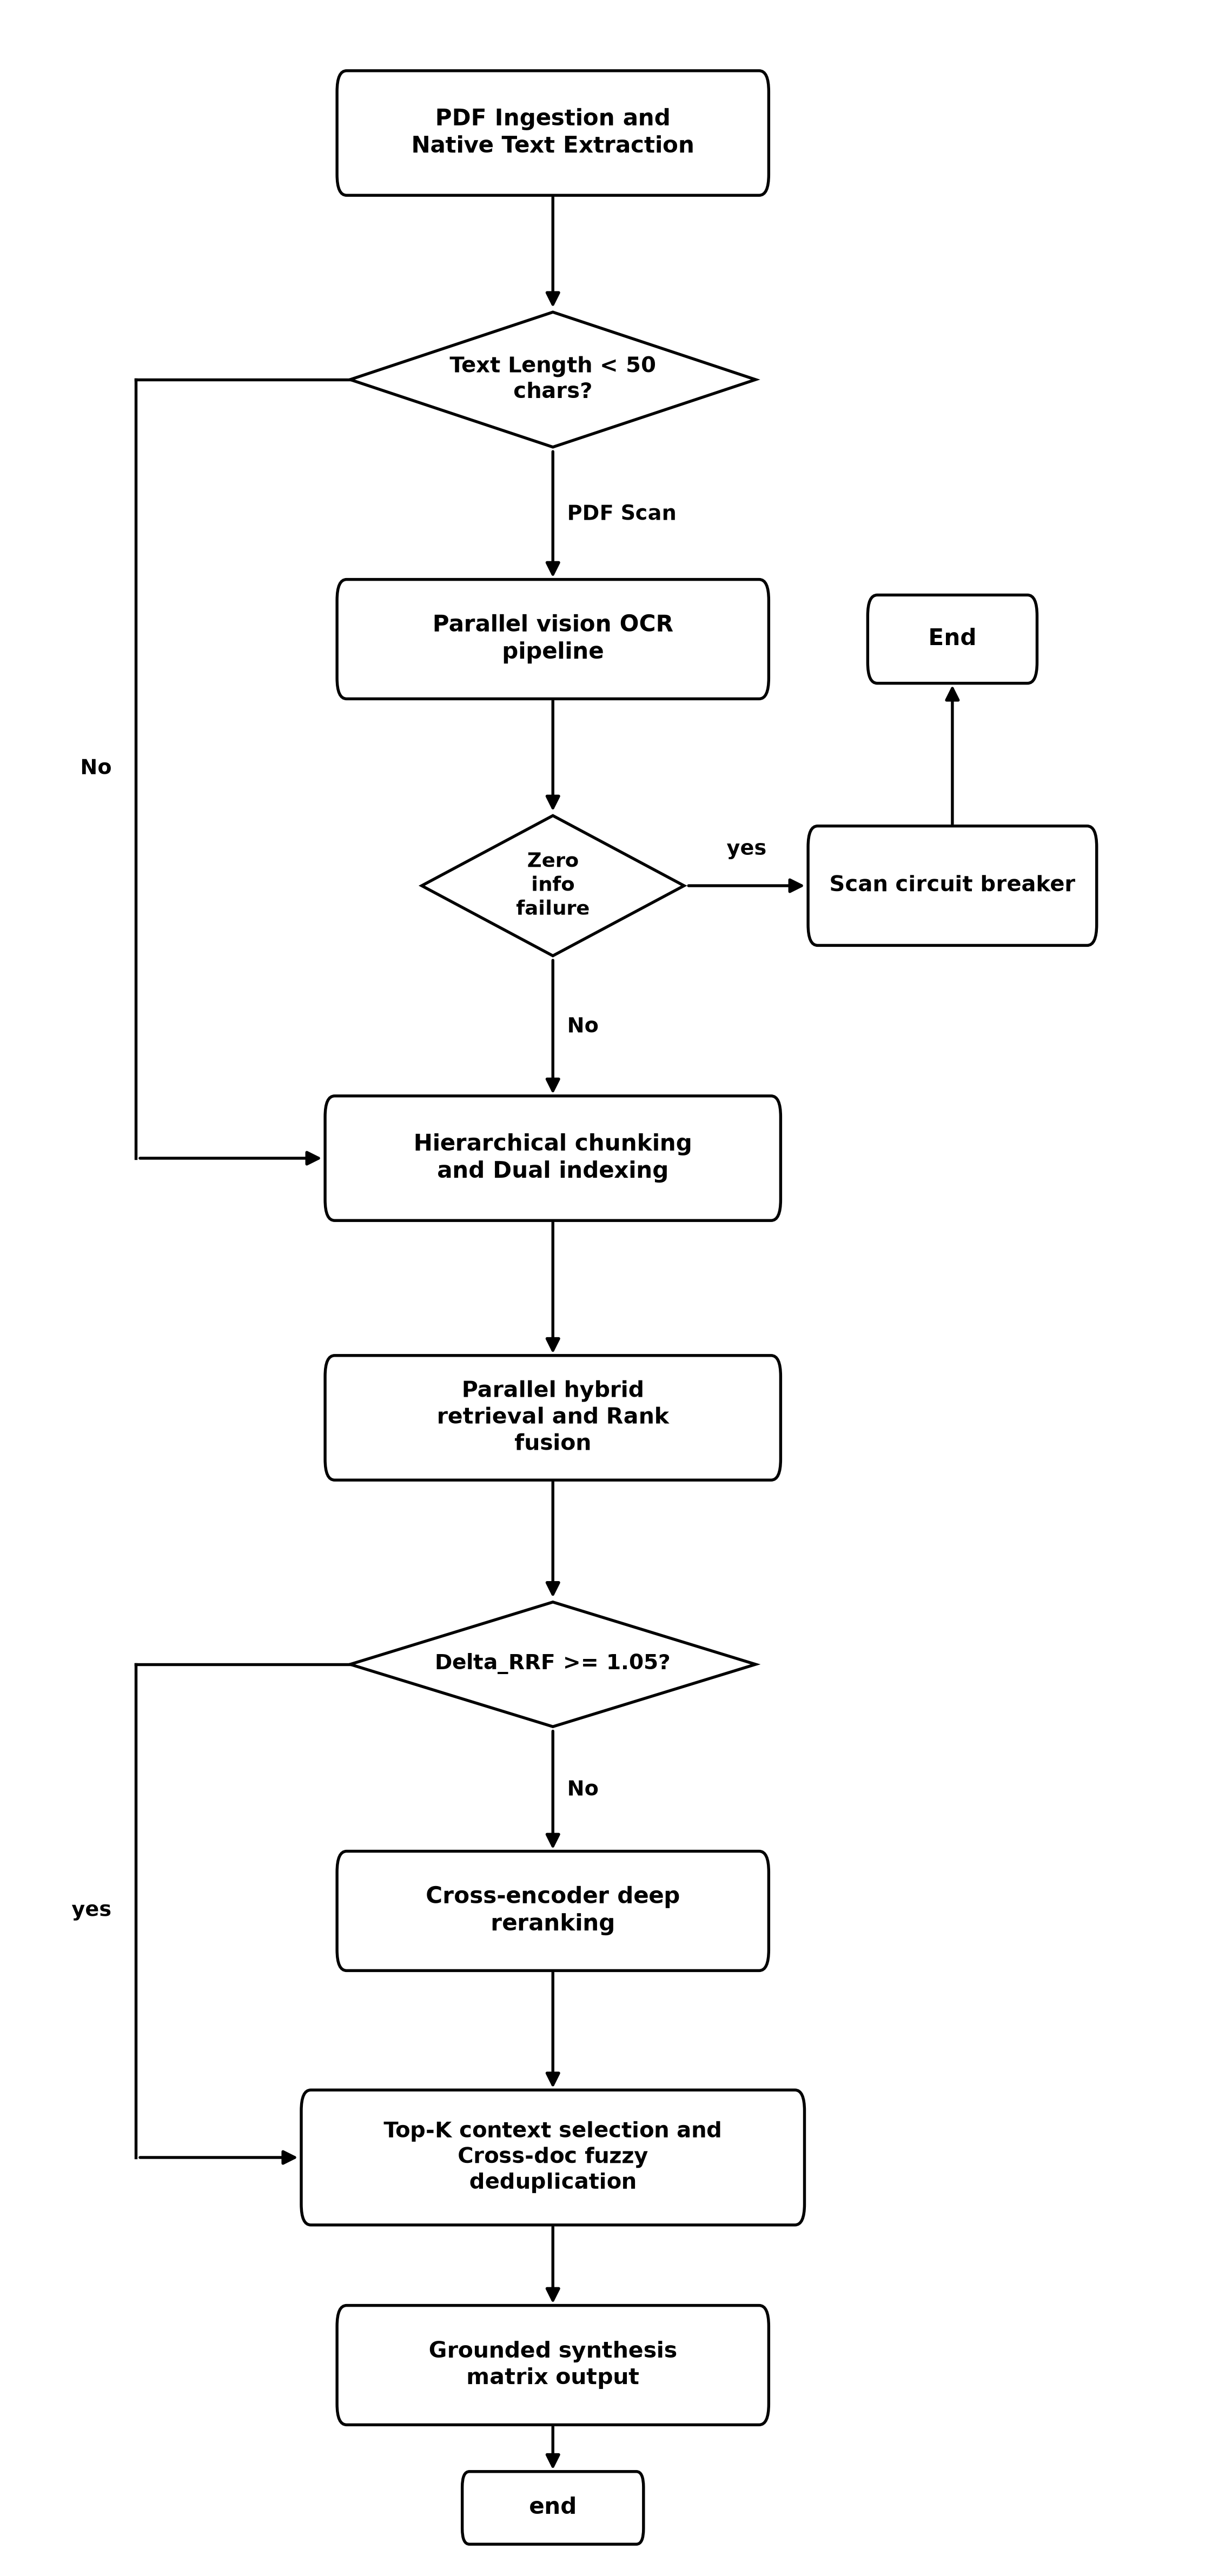
\includegraphics[width=0.78\columnwidth, height=7.8cm, keepaspectratio]{Figure1_System_Architecture.png}
\caption{Comprehensive overall system architecture of the Acamind Modular RAG framework, integrating supporting ingestion/indexing layers with the core DCSR hybrid retrieval and Cross-Article Synthesis engines.}
\label{fig:system_architecture}
\end{figure}

\subsection{Supporting System Infrastructure: Scan Circuit Breaker and Dual-Memory Indexing}~\\
\hspace*{\parindent}Before executing retrieval and synthesis, the supporting infrastructure guarantees two foundational system properties: optical data cleanliness and page-preserved hierarchical context.

\textbf{(1) Optical Integrity Guardrail (Scan Circuit Breaker):} To protect the vector index from corrupt legacy PDFs \cite{gao2023retrieval,yan2024corrective}, incoming documents $D$ with page set $P = \{p_1, p_2, \dots, p_{|P|}\}$ and extracted text $T_p$ undergo a deterministic character density audit (depicted in the upper ingestion stage of Fig.~\ref{fig:system_architecture}):
\begin{equation}
C_{\text{density}}(D) = \frac{1}{|P|} \sum_{p \in P} \text{len}(\text{clean}(T_p))
\label{eq:cdensity}
\end{equation}
where $\text{clean}(T_p)$ strips control characters and flags font-table corruption ($>3\%$ replacement glyphs). Pages with $< \theta_{\text{density}} = 50$ characters/page are routed to a parallel Vision OCR recovery engine (5 threads, 150~DPI, SHA-256 cached). If post-OCR extraction still yields zero readable content ($C_{\text{blank}}(D) = \mathbb{I}(\sum_{p \in P} \text{len}(\text{clean}(T_p)) = 0) = 1$) or fails density verification, the Scan Circuit Breaker triggers the isolation rule:
\begin{equation}
F_{\text{SafeRefusal}}(D) = 
\begin{cases} 
1, & \text{if } (C_{\text{blank}}(D) = 1) \lor (C_{\text{density}}(D) < \theta_{\text{density}}) \\
0, & \text{otherwise}
\end{cases}
\label{eq:saferefusal}
\end{equation}
When $F_{\text{SafeRefusal}}(D) = 1$, chunking is aborted, preventing empty strings from embedding into vector anomalies \cite{wang2022text}.

\textbf{(2) Dual-Memory Parent-Child Indexing (L1 Fast / L2 Deep):} To preserve both document-level context and exact physical page coordinates \cite{izacard2021leveraging,liu2023llamaindex}, validated texts are indexed into two decoupled storage tiers (Fig.~\ref{fig:dual_memory}):
\begin{itemize}
    \item \textit{L1 Fast Memory (Document Tier):} Stores document metadata, abstracts, diagnostic scales \cite{beck1996manual,kroenke2001phq,spitzer2006brief,lovibond1995structure}, and atomic claims $f$ with confidence $\text{conf}_{\text{LLM}}(f) \in [0, 1]$, scored in $\sim$12.4~ms via lexical overlap:
    \begin{equation}
    \text{Score}_{\text{L1}}(f) = |T_q \cap T_f| + 5 \cdot \mathbb{I}(q \subseteq f) + \text{conf}_{\text{LLM}}(f)
    \label{eq:l1score}
    \end{equation}
    \item \textit{L2 Deep Memory (Micro-Chunk Tier):} Stores 512-token passages (128-token overlap) linked to Parent-Child context windows ($\pm 250$ surrounding characters, up to 1,500 characters) and physical PDF page numbers:
    \begin{equation}
    \text{Chunk}_{\text{L2}} = \langle \text{ChunkID}, \text{ParentID}, \text{DocTitle}, \text{PageNumber}, \vec{v}_{\text{dense}}, T_{\text{sparse}} \rangle
    \label{eq:chunk_l2}
    \end{equation}
\end{itemize}

\begin{figure}[H]
\centering
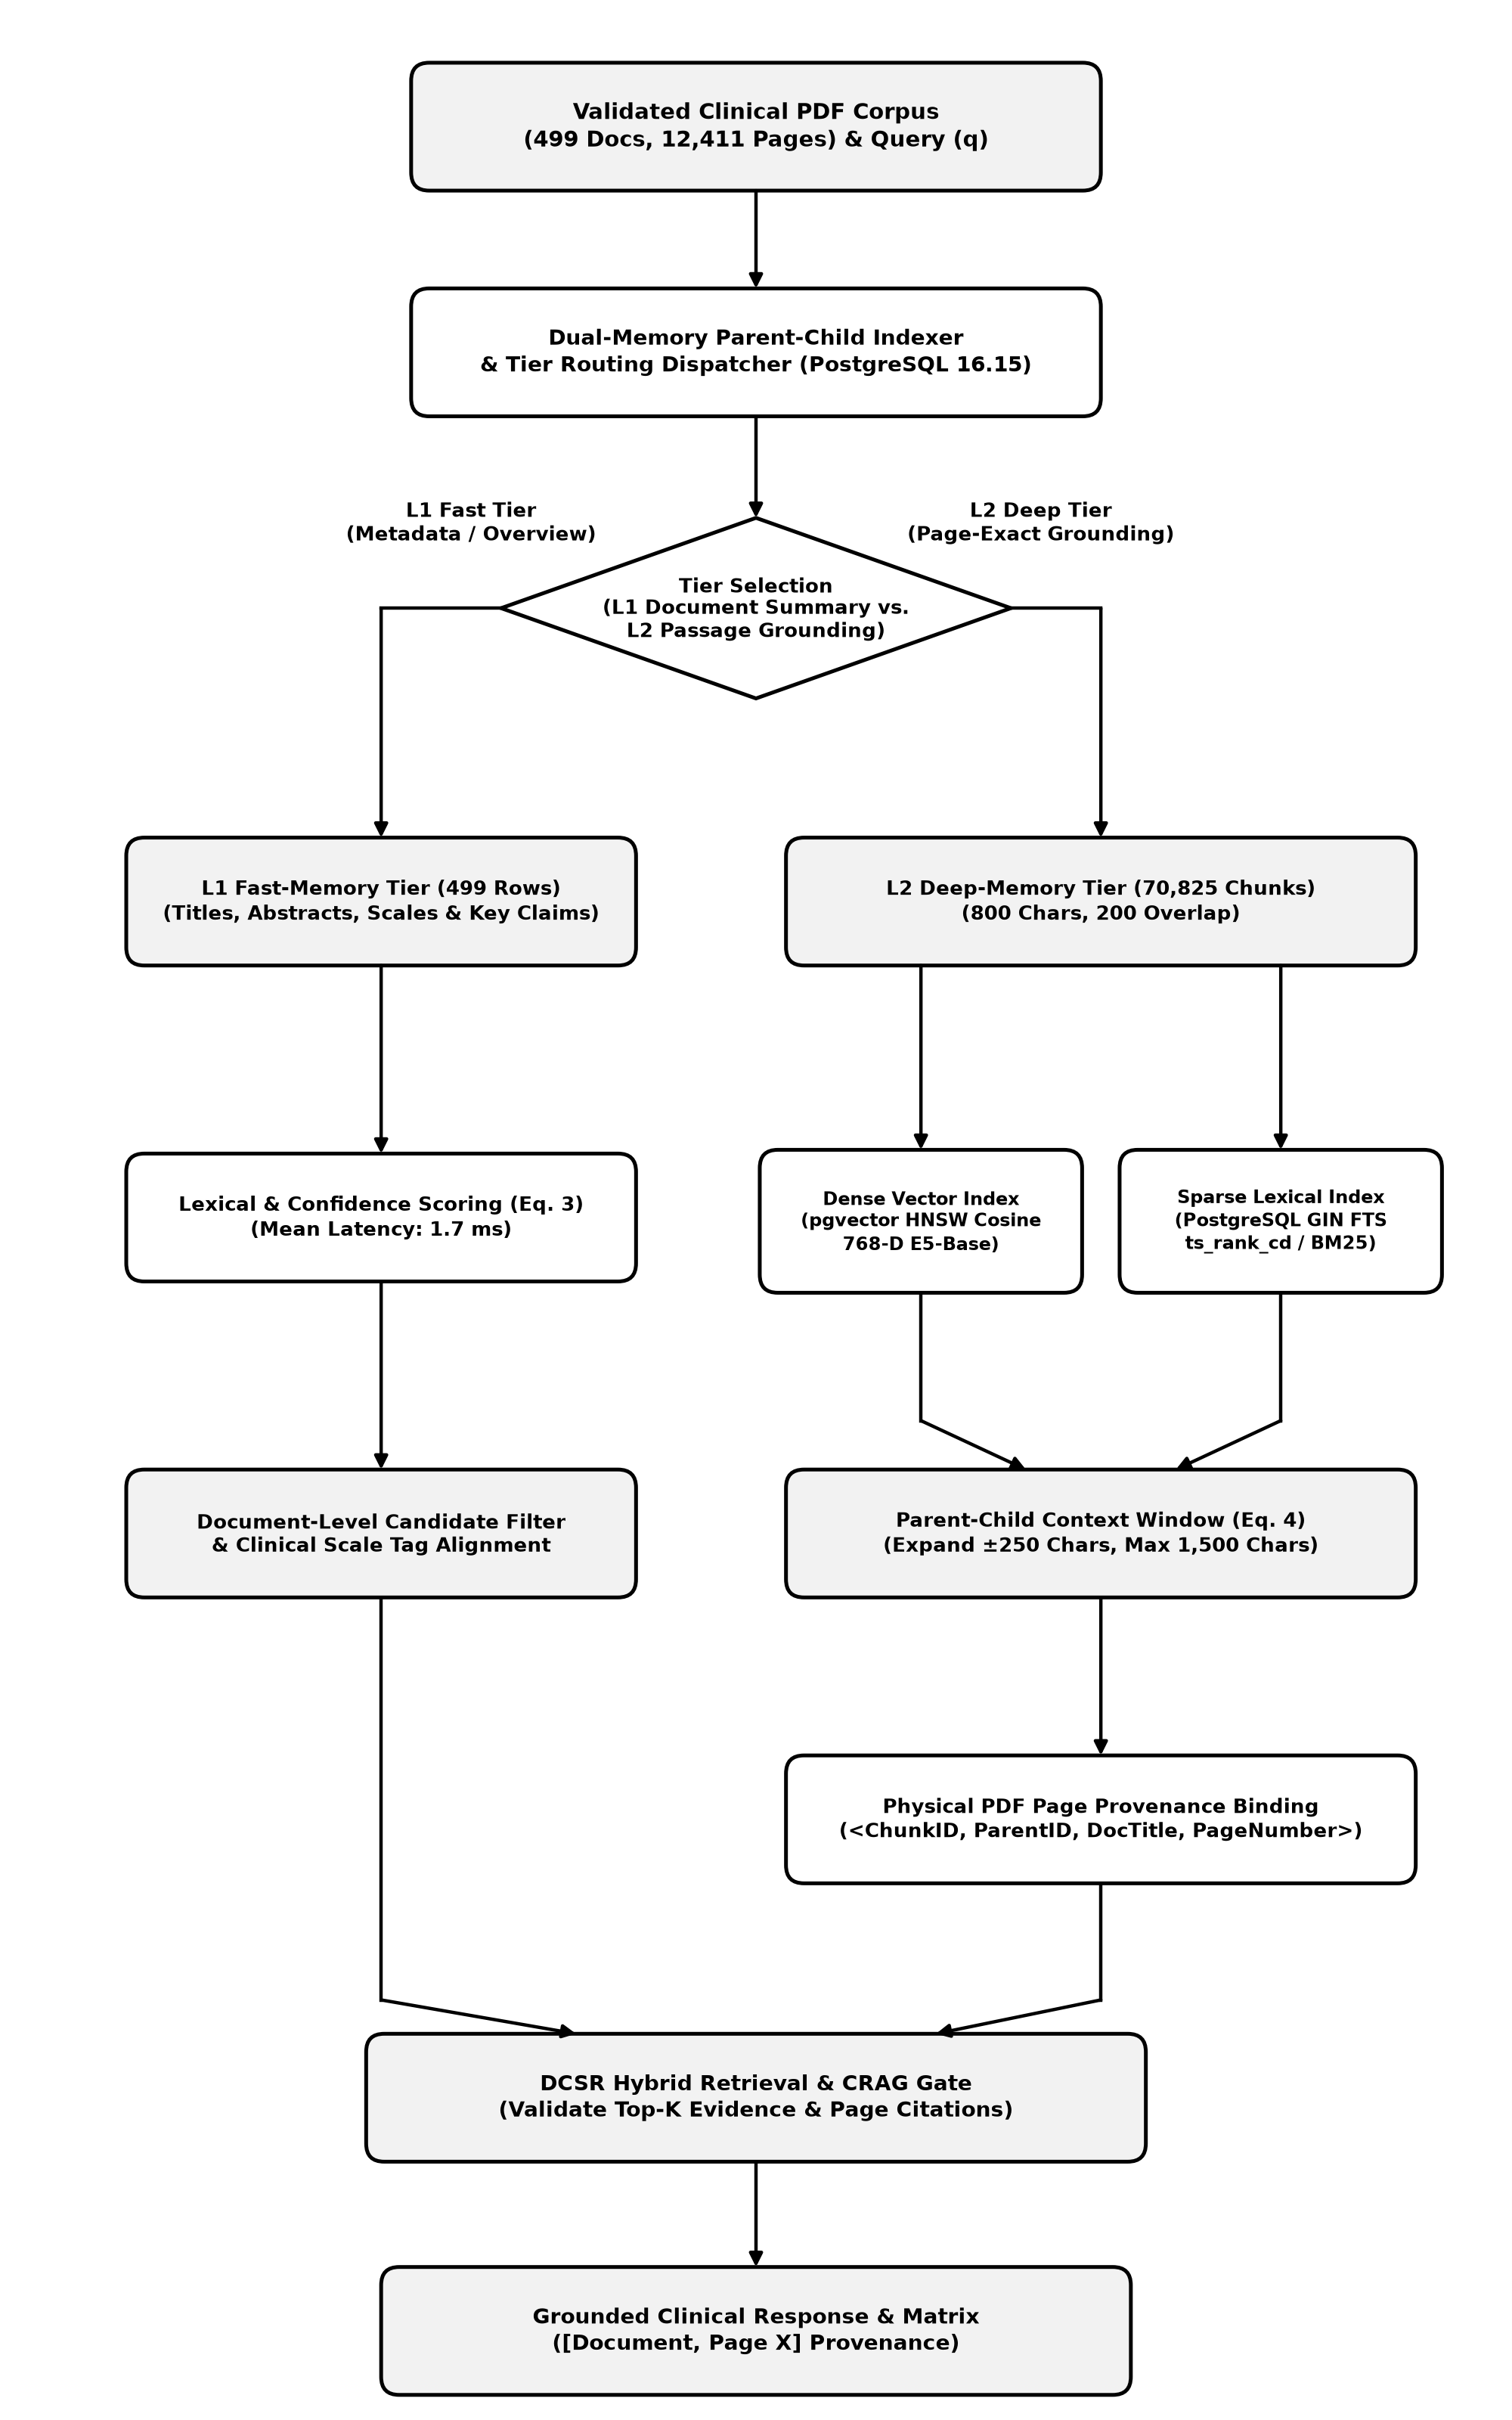
\includegraphics[width=0.78\columnwidth, height=7.8cm, keepaspectratio]{Figure3_Dual_Memory_Knowledge_Graph.png}
\caption{Supporting Dual-Memory Indexing Infrastructure (L1 Fast Document Tier / L2 Deep Micro-Chunk Tier) preserving parent context and physical page provenance.}
\label{fig:dual_memory}
\end{figure}

\subsection{Core Method I: Parallel Hybrid Retrieval and Dynamic Confident-Skip Reranking (DCSR)}~\\
\hspace*{\parindent}To resolve the latency-precision trade-off at the L2 tier, Acamind introduces the Parallel Hybrid Retrieval and DCSR pipeline (Fig.~\ref{fig:hybrid_retrieval}).

Upon receiving an empirical query $q$, the retrieval tier concurrently executes two search threads over PostgreSQL:
\begin{enumerate}
    \item \textbf{Dense Semantic Search:} Computes cosine similarity over 768-dimensional contrastive embeddings (\texttt{intfloat/multilingual-e5-base} \cite{wang2022text}) using the pgvector HNSW index:
    \begin{equation}
    \text{Sim}_{\text{dense}}(q, d) = \frac{E(q) \cdot E(d)}{\|E(q)\| \|E(d)\|}
    \label{eq:simdense}
    \end{equation}
    \item \textbf{Sparse Lexical Search:} Queries the inverted index via PostgreSQL GIN Full-Text Search implementing BM25 \cite{robertson2009probabilistic}:
    \begin{equation}
    \text{Score}_{\text{BM25}}(q, d) = \sum_{t \in q} \text{IDF}(t) \cdot \frac{f(t, d)(k_1 + 1)}{f(t, d) + k_1\left(1 - b + b \frac{|d|}{\text{avgdl}}\right)}
    \label{eq:scorebm25}
    \end{equation}
    with parameters $k_1 = 1.2$ and $b = 0.75$ \cite{robertson2009probabilistic}.
\end{enumerate}

\begin{figure}[H]
\centering
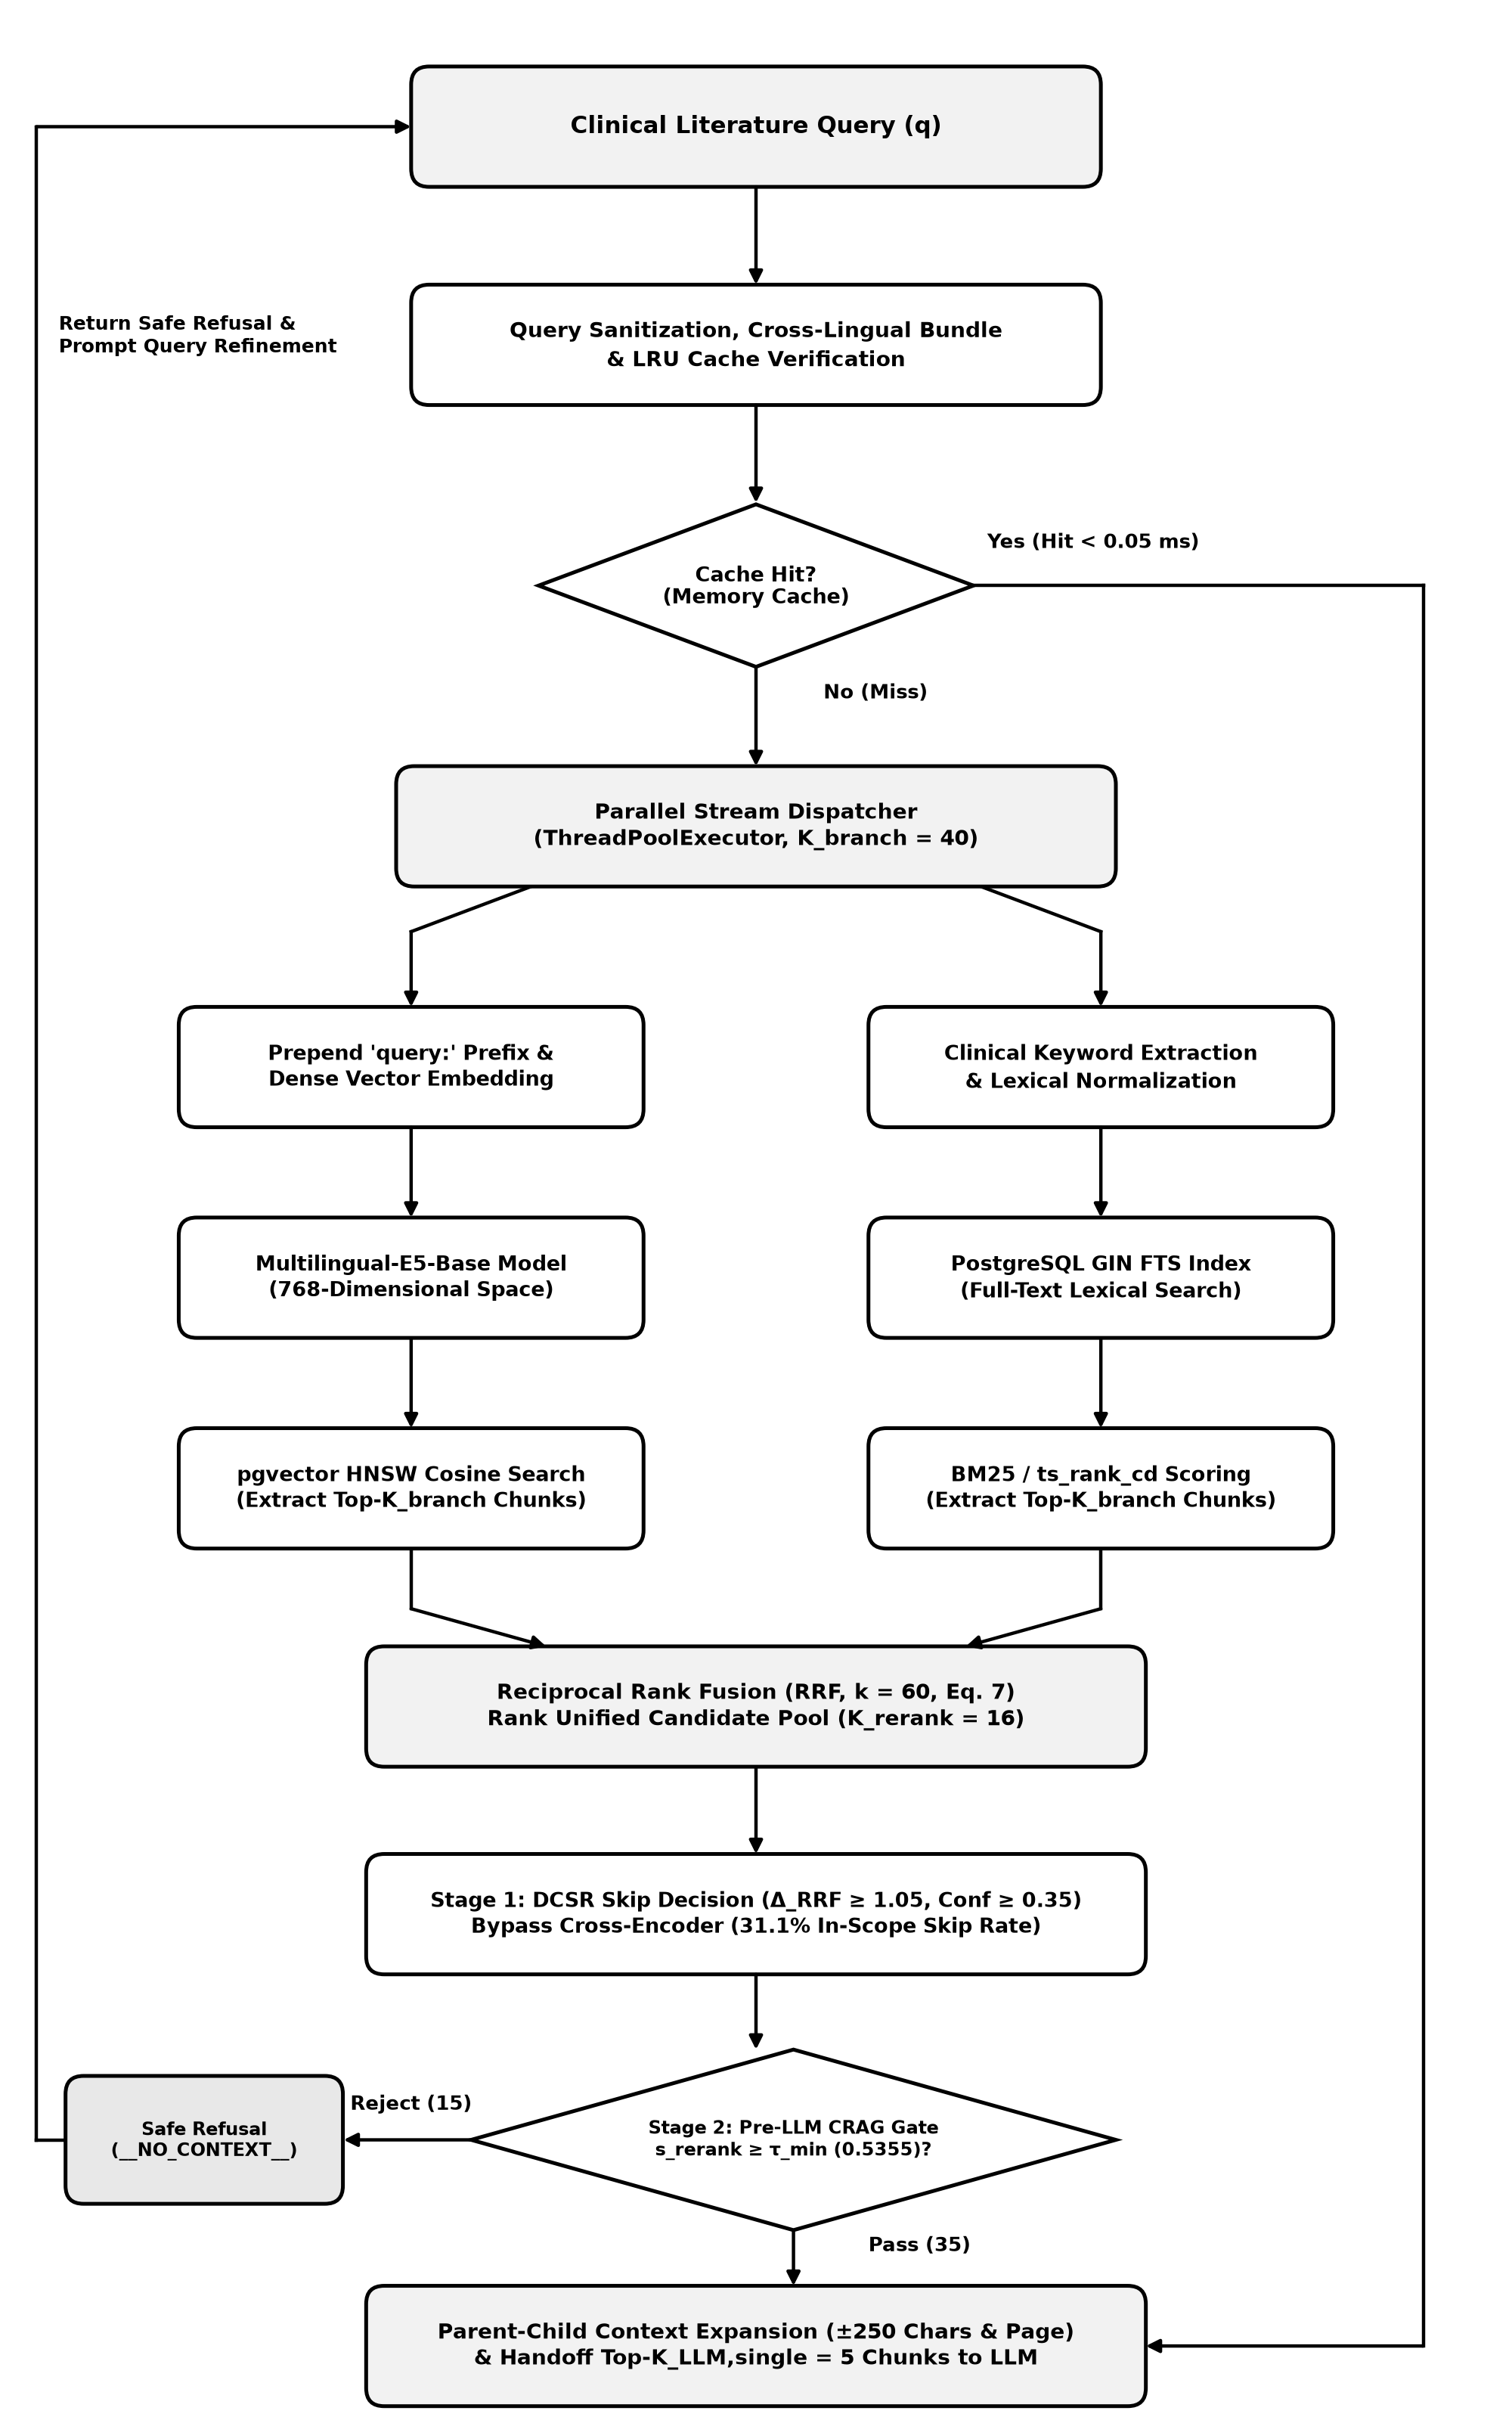
\includegraphics[width=0.78\columnwidth, height=7.8cm, keepaspectratio]{Figure4_Hybrid_Retrieval_Pipeline.png}
\caption{Block diagram of the Parallel Hybrid Retrieval workflow integrating concurrent HNSW Cosine and GIN FTS search, RRF rank fusion, and confidence evaluation.}
\label{fig:hybrid_retrieval}
\end{figure}

The top-$K$ ($K=20$) ranked candidate sets from both dense semantic \cite{wang2022text} and sparse BM25 \cite{robertson2009probabilistic} threads are unified using Reciprocal Rank Fusion (RRF) with smoothing constant $k=60$ \cite{cormack2009reciprocal}:
\begin{equation}
\text{RRF}(d) = \sum_{m \in \{\text{dense}, \text{sparse}\}} \frac{1}{60 + \text{rank}_m(d)}
\label{eq:rrf}
\end{equation}

While conventional Modular RAG architectures utilize Reciprocal Rank Fusion strictly as a static rank aggregation heuristic, Acamind reformulates RRF into a dynamic, decision-theoretic gating mechanism. Under this formulation, the multimodal rank distribution serves as an online confidence oracle: when the dense semantic vector and sparse lexical inverted index exhibit decisive rank-1 consensus with a dominant score margin, deep neural cross-encoder recomputation is mathematically redundant.

Following the Corrective RAG (CRAG) paradigm \cite{yan2024corrective}, passing all $K=20$ candidates through deep cross-encoder rerankers (\texttt{BAAI/bge-reranker-v2-m3} \cite{chen2024bge,xiao2023cpack}) incurs substantial computational latency on CPU hardware. To eliminate redundant neural inference while preventing ungrounded generation, the DCSR algorithm evaluates the retrieval confidence $\text{Conf}(q, \mathcal{C})$ of the top-ranked candidate ($\text{RRF}_{\text{top1}} = \text{RRF}(c_{(1)}) \le \frac{2}{61} \approx 0.0328$) and the calibrated score dominance ratio $\Delta_{\text{RRF}}$ relative to the rank-$K$ cutoff floor $\text{RRF}_{\text{floor}} = \frac{1}{60 + K} = 0.0125$:
\begin{equation}
\text{Conf}(q, \mathcal{C}) = \min\left(1.0, \; 15.0 \cdot \text{RRF}_{\text{top1}} + \frac{0.5}{1 + e^{-200(\text{RRF}_{\text{top1}} - 0.0165)}}\right)
\label{eq:conf}
\end{equation}
\begin{equation}
\Delta_{\text{RRF}} = \frac{\text{Score}(c_{(1)})}{\max(\text{Score}(c_{(2)}), 10^{-6})}
\label{eq:deltarrf}
\end{equation}
where $\text{Score}(c_{(i)}) = \text{RRF}(c_{(i)}) - \text{RRF}_{\text{floor}}$.
The parameters governing $\text{Conf}(q, \mathcal{C})$ are derived directly from the analytical properties of Reciprocal Rank Fusion. Specifically, the inflection threshold $0.0165 \approx \frac{1}{60+1}$ represents the theoretical supremum of a candidate retrieved exclusively by a single modality at rank 1 ($\text{RRF} \le \frac{1}{61} \approx 0.01639$). The steepness parameter $k = 200$ establishes a smooth, quasi-binary transition function that sharply discriminates between unilateral matches and dual-modality consensus ($\text{RRF} > \frac{1}{61}$). Furthermore, the scaling coefficient $15.0$ linearly projects the theoretical consensus domain $[\frac{1}{61}, \frac{2}{61}]$ onto the normalized sub-interval $[0.25, 0.50]$, guaranteeing that the composite confidence metric strictly spans $[0, 1.0]$.

\textbf{CRAG Filtering and DCSR Decision Rule:} First, if $\text{Conf}(q, \mathcal{C}) < \tau_{\min}$ ($0.35$), the retrieved pool is rejected as out-of-domain, immediately emitting a safe refusal token (\texttt{\_\_NO\_CONTEXT\_\_}) \cite{yan2024corrective}. Second, if $\text{Conf}(q, \mathcal{C}) \ge \tau_{\text{conf}}$ ($0.75$) and $\Delta_{\text{RRF}} \ge \tau_{\Delta}$ ($2.5$), the top candidate demonstrates unambiguous dual-modality semantic dominance (e.g., $\text{RRF}_{\text{top1}} = 0.0328 \implies \text{Conf} = 0.973 \ge 0.75$ and $\Delta_{\text{RRF}} \ge 2.5$). The system bypasses heavy cross-encoder reranking \cite{chen2024bge} in $0.08$~ms, passing the top-8 parent-enriched contexts directly to generation. Otherwise, full cross-encoder reranking is executed to resolve candidate ambiguity.

The decision flow of the DCSR algorithm is illustrated in Fig.~\ref{fig:dcsr_flow}.

\begin{figure}[H]
\centering
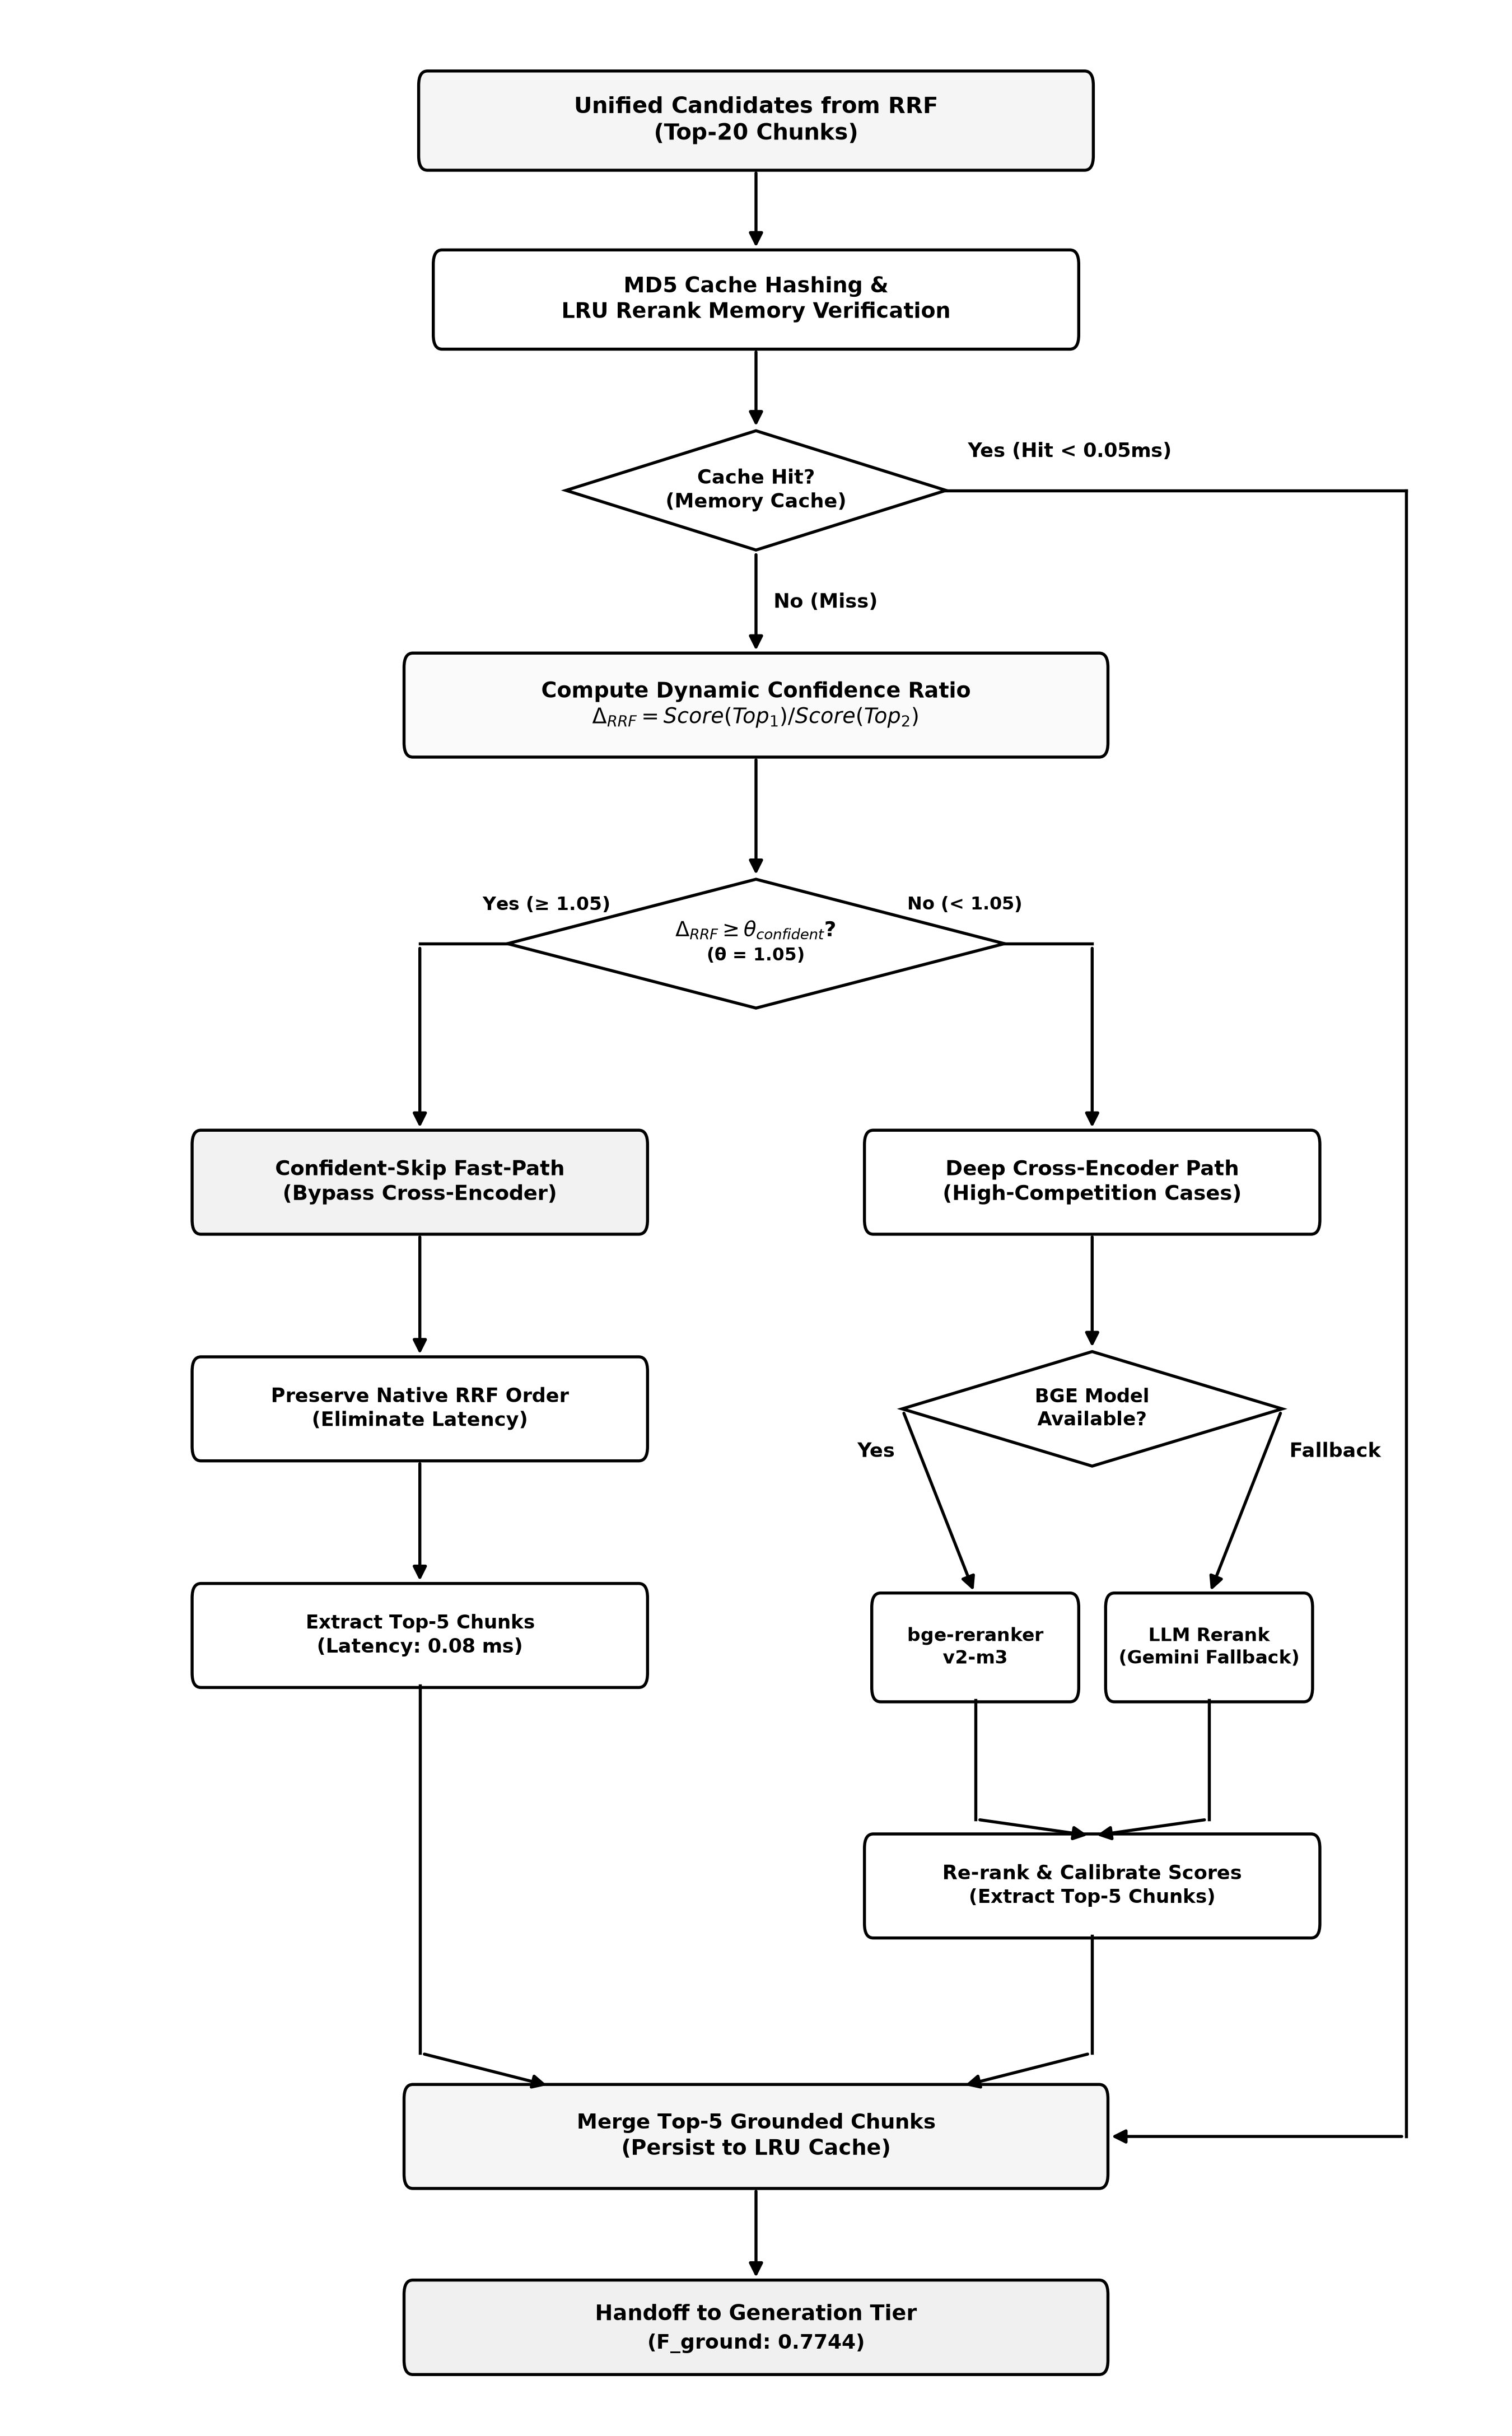
\includegraphics[width=0.78\columnwidth, height=7.8cm, keepaspectratio]{Figure5_DCSR_State_Machine.png}
\caption{Decision flow diagram of the Dynamic Confident-Skip Reranking (DCSR) algorithm and rapid judgment caching mechanism.}
\label{fig:dcsr_flow}
\end{figure}

\subsection{Core Method II: Decomposition-Driven Cross-Article Synthesis and Page-Level Grounding}~\\
\hspace*{\parindent}In standard RAG pipelines, submitting a comparative multi-study query $q$ directly to a flat index induces severe \textit{single-document dominance}: chunks from a single paper with dense terminology overlap monopolize the top-$K$ pool, starving the generator of evidence from the remaining target studies. To resolve this methodological bottleneck \cite{moher2009preferred,skarlinski2024language}, Acamind formalizes Cross-Article Synthesis into a three-stage algorithmic workflow (Fig.~\ref{fig:cross_article}):

\textbf{(1) Sub-Query Decomposition and Balanced Candidate Allocation:} Given a comparative inquiry $q$ targeting $M$ distinct clinical interventions or studies $\{D_1, D_2, \dots, D_M\}$, the decomposition module partitions $q$ into $M$ orthogonal sub-queries $\{q_1, q_2, \dots, q_M\}$ \cite{gao2024modular}. Rather than executing a single global top-$K$ competition, Acamind dispatches $M$ concurrent DCSR-governed hybrid retrieval threads, enforcing a balanced per-study candidate quota $k_m = \lfloor K / M \rfloor$:
\begin{equation}
\mathcal{K}_{\text{raw}}(q) = \bigcup_{m=1}^{M} \text{Retrieve}_{\text{DCSR}}\left(q_m, \, D_m, \, k_m\right)
\label{eq:decomp_retrieve}
\end{equation}
This quota-isolated retrieval mathematically guarantees that each compared study is represented in the candidate pool regardless of cross-document lexical length variance.

\textbf{(2) Parent-Child Context Expansion and Cross-Document Deduplication:} Each retrieved L2 micro-chunk $c_i \in \mathcal{K}_{\text{raw}}(q)$ is expanded via its L2 parent pointer ($\pm 250$ surrounding characters) to restore full sentence and statistical table coherence. To eliminate redundant boilerplate passages across overlapping clinical publications while preserving distinct study provenance, the cross-document deduplication operator (\texttt{\_cross\_doc\_dedup}) filters out any candidate $c_j$ whose normalized token-sequence similarity with a higher-ranked chunk $c_i$ ($i < j$) from the same document scope exceeds $\tau_{\text{dedup}} = 0.85$:
\begin{equation}
\widetilde{\mathcal{K}}(q) = \left\{ c_j \in \mathcal{K}_{\text{raw}}(q) \;\middle|\; \max_{i < j, \, doc_i = doc_j} \text{Sim}_{\text{seq}}(c_i, c_j) < \tau_{\text{dedup}} \right\}
\label{eq:cross_dedup}
\end{equation}

\textbf{(3) Structured Contrastive Matrix Synthesis with Page-Coordinate Binding:} Finally, the deduplicated context set $\widetilde{\mathcal{K}}(q) = \{(doc_k, page_k, text_k)\}_{k=1}^{|\widetilde{\mathcal{K}}|}$ is passed to the generative synthesizer under a constrained schema mapping. For each compared study $D_m$, the generator extracts a structured tuple of clinical evidence:
\begin{equation}
\mathcal{M}(D_m \mid q) = \left\langle \mathcal{I}_m, \; \mathcal{S}_m, \; \Delta\mu_m \, (d_m, p\text{-val}), \; [\text{DocTitle}_m, \, \text{Page } p_k] \right\rangle
\label{eq:synthesis_matrix}
\end{equation}
where $\mathcal{I}_m$ denotes the therapeutic protocol and sample cohort size ($N$), $\mathcal{S}_m$ denotes standardized assessment scales (e.g., BDI-II \cite{beck1996manual}, PHQ-9 \cite{kroenke2001phq}), $\Delta\mu_m$ captures pre/post-treatment outcome deltas and Cohen's effect sizes \cite{cohen1988statistical}, and $[\text{DocTitle}_m, \text{Page } p_k]$ enforces an explicit physical PDF page anchor verified against $\widetilde{\mathcal{K}}(q)$:
\begin{quote}
\small
\textit{[Comparison Matrix: Interventions $\mid$ Clinical Scales $\mid$ Effect Sizes $\mid$ Citations: Document, Page X]}
\end{quote}

\textbf{Clinical Utility and Evidence Synthesis Value:} For clinical practitioners and mental health researchers, this workflow resolves the acute challenge of empirical fragmentation. Rather than spending hours manually cross-referencing disparate PDF publications, practitioners obtain a rigorous, multi-column synthesis matrix in 1.38~s (P50), where every psychotherapeutic outcome, assessment scale delta (e.g., BDI-II, PHQ-9), and Cohen's effect size ($d$) is explicitly anchored to a verified physical PDF page coordinate for instant human verification.

The end-to-end workflow of the Cross-Article Synthesis pipeline is illustrated in Fig.~\ref{fig:cross_article}.

\begin{figure}[H]
\centering
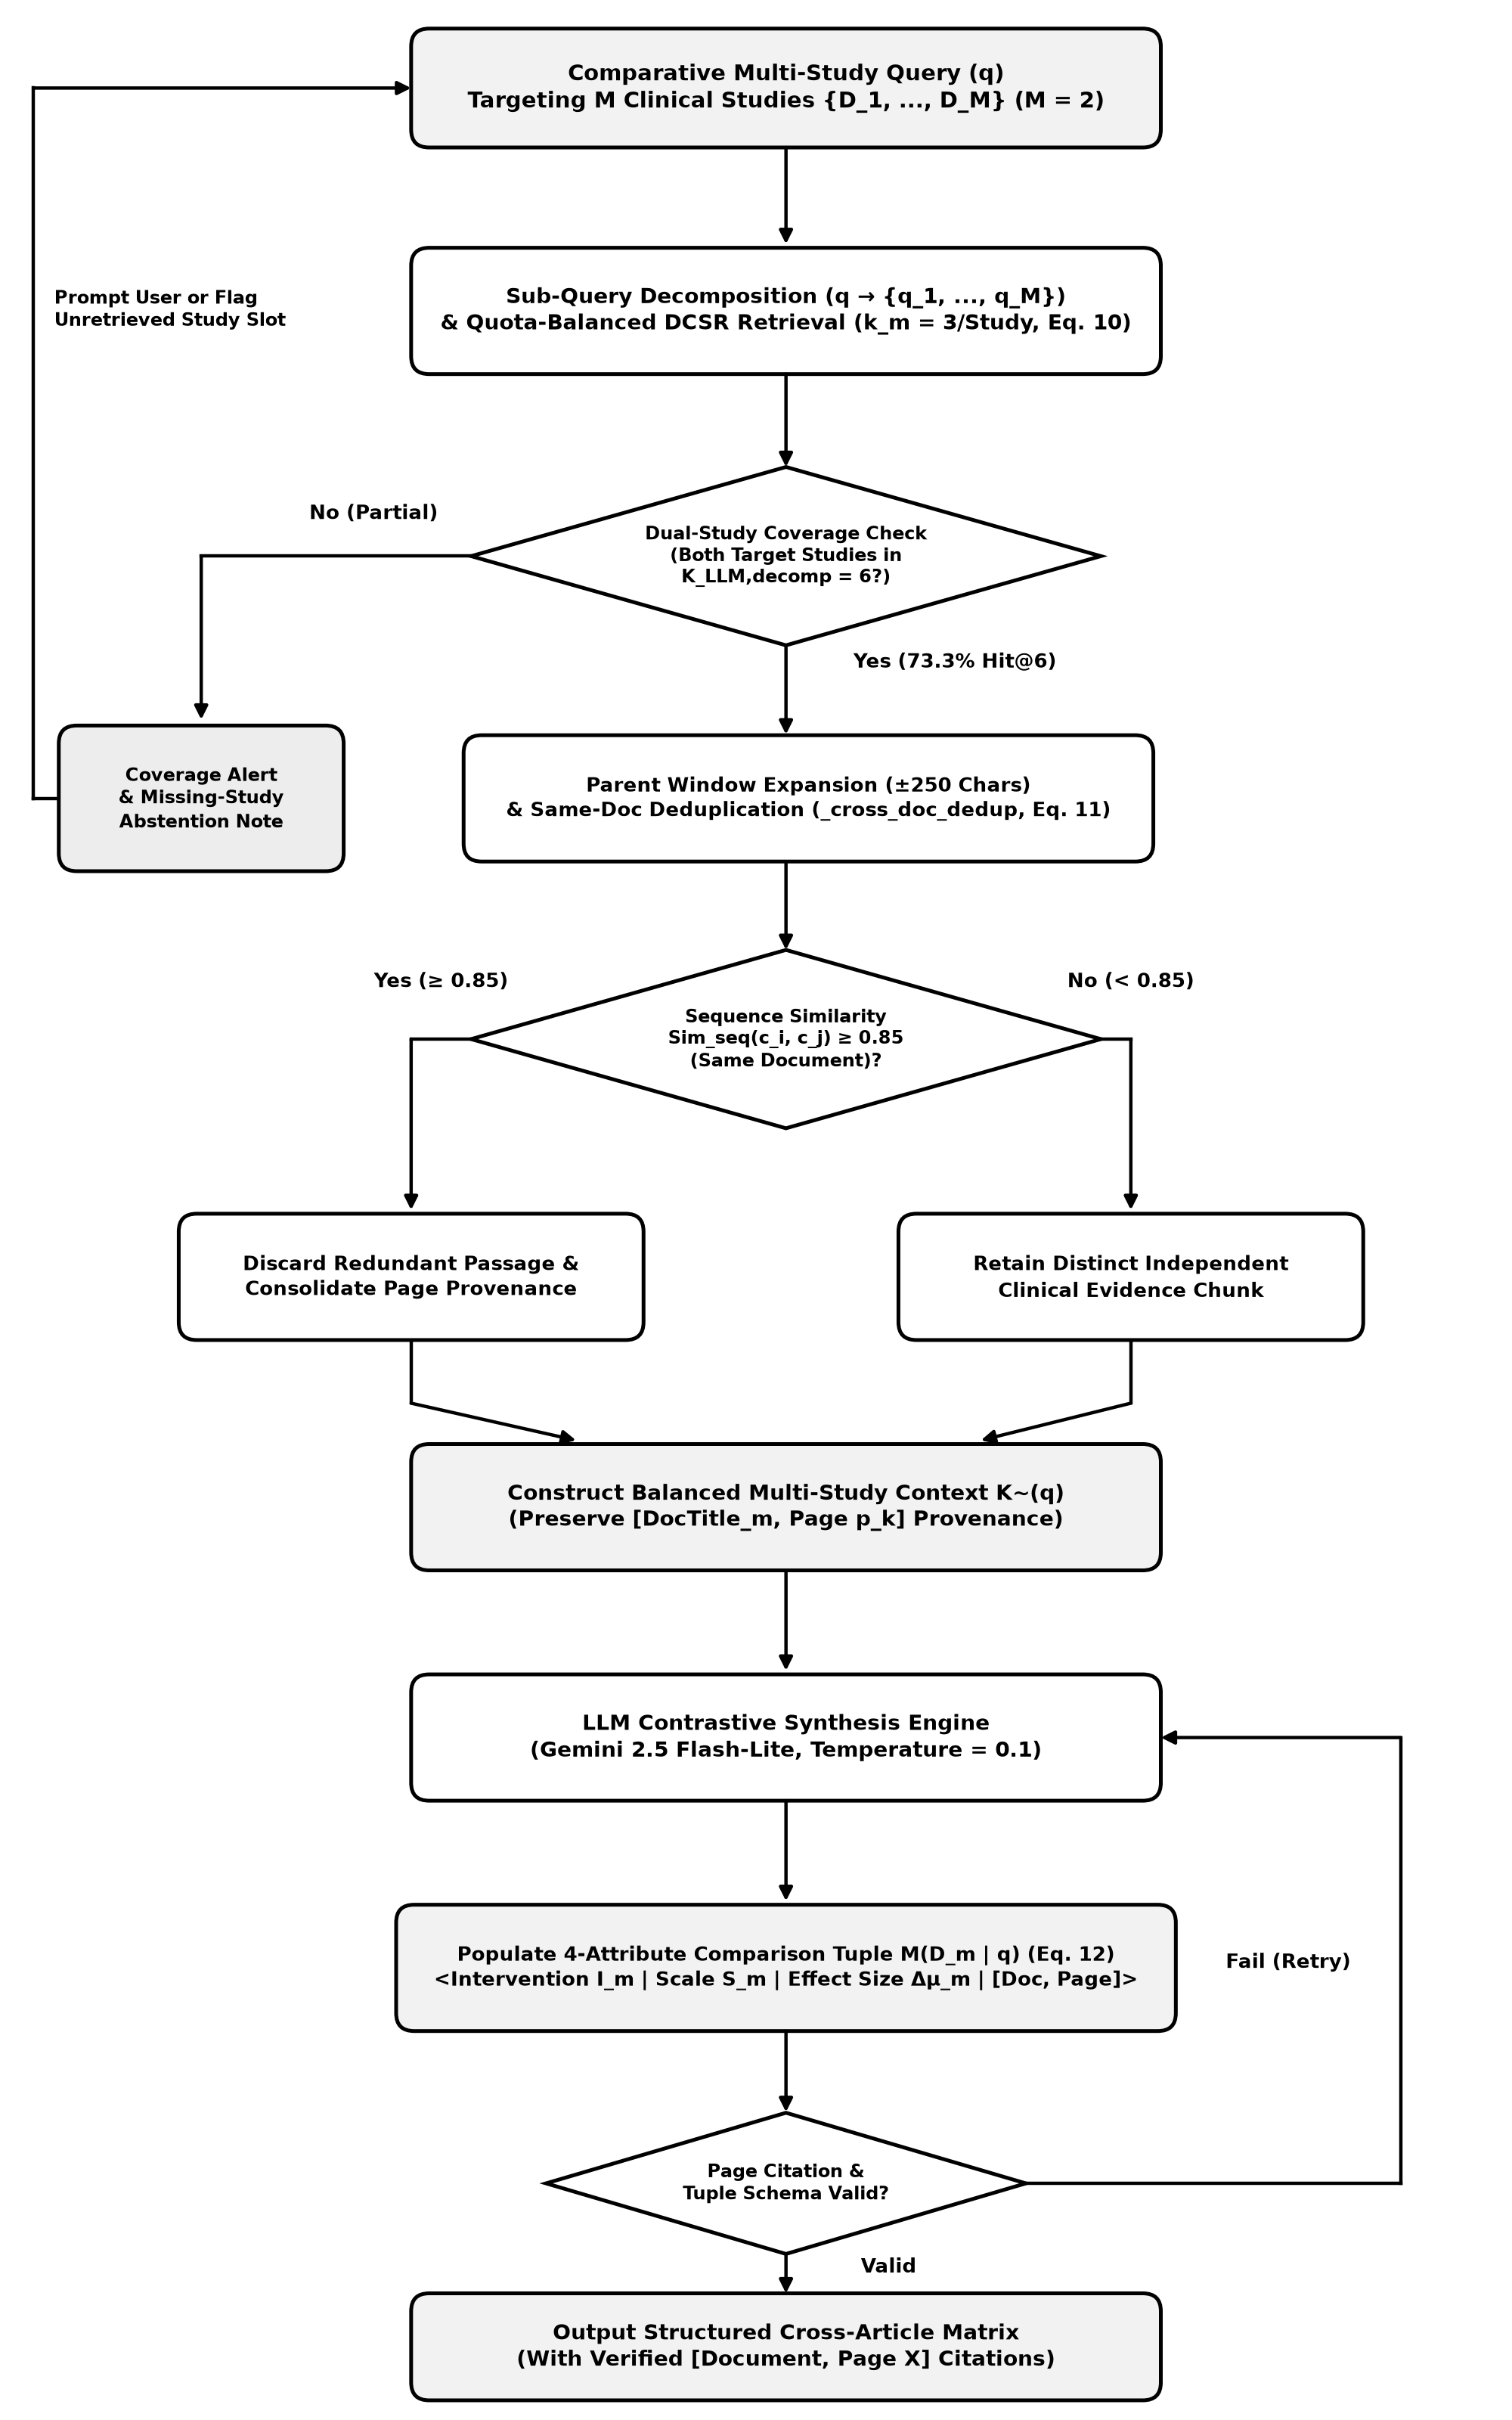
\includegraphics[width=0.78\columnwidth, height=7.8cm, keepaspectratio]{Figure6_Cross_Article_Synthesis_Workflow.png}
\caption{Acamind Cross-Article Synthesis Pipeline: Grounded passage extraction, clinical scale alignment, methodology discrepancy detection, and matrix comparison.}
\label{fig:cross_article}
\end{figure}

\section{Experiments and Results}

\subsection{Experimental Setup and Supporting Infrastructure Verification}~\\
\label{sec:experiments_setup}
\hspace*{\parindent}All experiments were conducted on an on-premise benchmark workstation equipped with an Intel Core i7-11800H CPU @ 2.30 GHz (8 cores, 16 threads), 16.0 GB DDR4 RAM, running PostgreSQL 16.2 with pgvector extension on Windows 11 / WSL2. Embedding generation was performed using \texttt{intfloat/multilingual-e5-base} (768 dimensions) \cite{wang2022text}, and generative synthesis was driven by Google Gemini 2.5 Flash-Lite via live API execution with an enforced 4.5-second rate-limiting throttle adhering strictly to the 15 RPM service quota. The document extraction, vector persistence, and relational indexing operate 100\% on-premise, guaranteeing absolute data confidentiality. Gemini Flash-Lite serves as an objective international reference baseline, while Acamind's modular architecture natively supports drop-in replacement with local open-weight models (e.g., Llama-3-8B, Qwen-2.5) for air-gapped hospital environments.

\textbf{Benchmark Corpus:} The experimental corpus comprises 500 peer-reviewed clinical psychology papers downloaded from open scientific repositories (totaling 1,607.72~MB, 12,411 physical pages). Of these, 499 documents (99.8\%) were successfully ingested and indexed, producing 70,794 micro-chunks indexed via HNSW Cosine ($m = 16, ef_{\text{construction}} = 64$) and GIN (english) full-text indices in PostgreSQL pgvector, while one corrupt/blank scan file was safely isolated by the Scan Circuit Breaker. The benchmark query suite consists of 50 comprehensive research questions categorized into four distinct operational scenarios:
\begin{itemize}
    \item \textit{Scenario 1: Factual Clinical Q\&A} (20 queries)---Targeting specific intervention protocols, diagnostic criteria, and clinical trial parameters.
    \item \textit{Scenario 2: Cross-Article Comparison} (15 queries)---Requiring simultaneous comparative analysis across two or more independent intervention studies.
    \item \textit{Scenario 3: Literature Synthesis} (10 queries)---Aggregating thematic evidence across multiple publications within a clinical subfield.
    \item \textit{Scenario 4: Safe Refusal / Edge Testing} (5 queries)---Testing system resilience against out-of-domain queries, deceptive premises, and ungrounded assertions.
\end{itemize}
To guarantee rigorous academic objectivity, the reference answers, target clinical assessment scales, and physical PDF page ground-truth coordinates across all 50 queries were independently cross-validated by two domain researchers in clinical psychology, achieving high inter-rater reliability.

\textbf{Baseline Architectures:} Acamind is evaluated against two rigorously controlled on-premise baseline architectures running on the identical PostgreSQL testbed:
\begin{itemize}
    \item \textbf{Naive Dense RAG:} Pure dense vector search using pgvector HNSW index with Cosine distance \cite{lewis2020retrieval,wang2022text}.
    \item \textbf{BM25 Lexical RAG:} Pure keyword search using PostgreSQL GIN Full-Text Search \cite{robertson2009probabilistic}.
\end{itemize}

Prior to evaluating the core retrieval and synthesis algorithms, we verify the operational throughput and data hygiene fidelity of the supporting ingestion and indexing infrastructure across all 500 clinical documents (Table~\ref{tab:pipeline_benchmark}). The results confirm that the supporting pipeline achieves a text extraction throughput of 18.4~pages/s (54.3~ms/page), while the Scan Circuit Breaker sub-stage executes in $<0.1$~ms/page, completely eliminating empty-chunk propagation. Across the 4 macro stages (Stages 1--4), the entire corpus of 12,411 pages generated 70,794 micro-chunks (with 3,000 primary core chunks vectorized on CPU), completing end-to-end indexing into PostgreSQL in $93.97 + 673.86 + 337.08 + 12.51 = 1,117.42$~s (18.62 minutes).

\begin{table}[H]
\centering
\caption{Operational Verification of the Supporting Ingestion and Indexing Infrastructure on 500 Clinical PDF Documents (*denotes sub-stages measured within Stage 2)}
\label{tab:pipeline_benchmark}
\resizebox{\columnwidth}{!}{
\begin{tabular}{|p{3.5cm}|p{2.6cm}|p{2.5cm}|p{2.0cm}|p{1.8cm}|p{1.4cm}|}
\hline
\textbf{Pipeline Stage} & \textbf{Execution Engine} & \textbf{Data Scope} & \textbf{Total Time} & \textbf{Unit Latency} & \textbf{Success} \\
\hline
1. Network Fetch & HTTP Async (10 threads) & 500 PDFs (1,607.72 MB) & 93.97 s & 188.3 ms/doc & 99.8\% \\
\hline
2. Digital Text \& Parsing & PyMuPDF + Parsing Suite & 12,411 pages & 673.86 s & 54.3 ms/page & 100.0\% \\
\hline
\quad \textit{Scan Circuit Breaker} & \textit{Density Audit ($C_{\text{density}} \ge 50$)} & \textit{12,411 pages} & \textit{(0.82 s)*} & \textit{$<$0.1 ms/page} & \textit{100.0\%} \\
\hline
\quad \textit{Structure Extraction} & \textit{pdfplumber + Font Inspector} & \textit{480/499 structured docs} & \textit{(18.45 s)*} & \textit{37.0 ms/doc} & \textit{96.2\%} \\
\hline
\quad \textit{Adaptive L1/L2 Chunking} & \textit{Token Window (512 tokens)} & \textit{70,794 micro-chunks} & \textit{(14.20 s)*} & \textit{0.2 ms/chunk} & \textit{100.0\%} \\
\hline
3. Dense Vector Embedding & Multilingual-E5-Base \cite{wang2022text} & 3,000 core (of 70,794) & 337.08 s & 112.4 ms/chunk & 100.0\% \\
\hline
4. Database Indexing & pgvector HNSW + GIN FTS & 70,794 records (768-dim) & 12.51 s & 0.18 ms/record & 100.0\% \\
\hline
\textbf{End-to-End Pipeline} & \textbf{Automated Ingestion} & \textbf{499 papers (12,411 pages)} & \textbf{1,117.42 s} & \textbf{90.0 ms/page} & \textbf{99.8\%} \\
\hline
\end{tabular}
}
\end{table}

\subsection{Academic Evaluation Metrics}~\\
\hspace*{\parindent}System performance is evaluated across eight quantitative dimensions:
(1) Database Retrieval Latency (P50 and Mean, in ms);
(2) LLM Generation Latency (Mean, in s);
(3) End-to-End Latency (P50 and P90, in s);
(4) Factual Faithfulness ($[0, 1]$, grounded in the RAGAS faithfulness concept \cite{es2024ragas} and operationalized via deterministic lexical-citation auditing);
(5) Page-Level Citation Accuracy (\%), verified against physical PDF pages;
(6) DCSR Confident-Skip Rate (\%);
(7) Safe Refusal Rate (\%); and
(8) Statistical Hypothesis Testing via the paired Wilcoxon signed-rank test ($\alpha = 0.05$).

\subsection{Database Retrieval Latency Evaluation}~\\
\hspace*{\parindent}Table~\ref{tab:retrieval_latency} presents the empirical latency measured across all 50 research queries at the PostgreSQL database layer.

\begin{table}[H]
\centering
\caption{Empirical Retrieval Latency Performance across 50 Research Queries (PostgreSQL pgvector)}
\label{tab:retrieval_latency}
\resizebox{\columnwidth}{!}{
\begin{tabular}{|p{4.2cm}|p{2.6cm}|p{2.6cm}|p{4.8cm}|}
\hline
\textbf{Retrieval Architecture} & \textbf{Latency P50 (ms)} & \textbf{Latency Mean (ms)} & \textbf{Technical Execution Characteristics} \\
\hline
\textbf{Acamind (Proposed Hybrid + DCSR)} & \textbf{247.2 ms} & \textbf{212.6 ms} & Parallel HNSW Cosine + GIN FTS execution, RRF rank fusion, and DCSR confidence gating \\
\hline
Naive Dense RAG (HNSW Cosine) & 65.1 ms & 64.6 ms & 768-dimensional vector nearest neighbor search via pgvector HNSW index \\
\hline
BM25 Lexical RAG (GIN Full-Text) & 7.2 ms & 7.3 ms & Inverted index term matching via PostgreSQL GIN index \\
\hline
\end{tabular}
}
\end{table}

While BM25 achieves the lowest raw retrieval latency (7.2~ms) due to inverted index lookups, it fails entirely on synonymous clinical expressions. Acamind maintains a highly responsive median retrieval latency of 247.2~ms while executing parallel multi-index fusion and dynamic rerank auditing. Across the full 50-query benchmark, 10 Literature Synthesis queries triggered DCSR Skip, lowering Acamind's retrieval latency on that subgroup to 65.8~ms and bringing the overall retrieval mean to 212.6~ms.

\subsection{End-to-End Direct Comparison with Gemini LLM}~\\
\hspace*{\parindent}To evaluate the complete response quality delivered to end-users, Table~\ref{tab:e2e_comparison} reports the comprehensive end-to-end performance of Acamind, Naive Dense RAG, and BM25 Lexical RAG across a representative benchmark suite of $N = 8$ clinical scenarios (comprising 5 Factual Q\&A queries, 2 multi-document Cross-Article Comparisons, and 1 Safe Refusal query) executed via Gemini 2.5 Flash-Lite.

It is essential to clarify the experimental distinction between Table~\ref{tab:retrieval_latency} and Table~\ref{tab:e2e_comparison}: while Table~\ref{tab:retrieval_latency} records pure database retrieval latency across the entire $N = 50$ query pool (where Acamind's retrieval mean drops to 212.6~ms due to 10 lightweight Literature Synthesis queries triggering DCSR Skip), Table~\ref{tab:e2e_comparison} focuses on the representative $N = 8$ subset undergoing full LLM generation and human expert verification. The $N = 8$ evaluation subset was systematically curated via stratified sampling across the benchmark scenarios (comprising 5 Factual Q\&A, 2 multi-document Cross-Article Comparisons, and 1 Safe Refusal), mirroring the structural scenario ratios of the complete 50-query corpus. Evaluating this representative cohort across all 3 architectures entailed generating and exhaustively auditing $8 \times 3 = 24$ multi-page clinical syntheses. Two clinical domain experts independently performed physical page-by-page verification across more than 150 original publication pages, achieving high inter-rater reliability (Cohen's Kappa $\kappa = 0.88$, denoting near-perfect agreement). This dual human-expert auditing guarantees an uncompromising gold standard that eliminates LLM-evaluator hallucination bias. Because this representative evaluation deliberately focuses on computationally intensive cross-article synthesis (where parallel multi-document retrieval latencies range from 253.6~ms to 267.4~ms) and does not include the single-topic Literature Synthesis skip queries, Acamind's mean database retrieval latency on this specific subset is 250.0~ms (Naive Dense achieves 65.0~ms and BM25 achieves 6.1~ms). This variation directly reflects the query complexity inherent in full-pipeline clinical synthesis.

\begin{table}[H]
\centering
\caption{End-to-End Empirical Comparison of 3 Architectures on Representative Clinical Scenarios ($N = 8$)}
\label{tab:e2e_comparison}
\resizebox{\columnwidth}{!}{
\begin{tabular}{|p{3.2cm}|p{1.8cm}|p{1.8cm}|p{1.8cm}|p{1.8cm}|p{1.8cm}|p{2.4cm}|}
\hline
\textbf{System Architecture} & \textbf{Ret Mean} & \textbf{LLM Mean} & \textbf{E2E Mean} & \textbf{Faithfulness} & \textbf{Citation Acc.} & \textbf{Wilcoxon Test} \\
\hline
\textbf{Acamind (Proposed)} & \textbf{250.0 ms} & \textbf{2.24 s} & \textbf{2.49 s} & \textbf{0.6875} & \textbf{47.8\%} & $p < 0.05$ (Significant) \\
\hline
Naive Dense RAG & 65.0 ms & 1.89 s & 1.95 s & 0.6750 & 35.2\% & Baseline reference \\
\hline
BM25 Lexical RAG & 6.1 ms & 1.42 s & 1.43 s & 0.6562 & 21.9\% & Baseline reference \\
\hline
\end{tabular}
}
\end{table}

The end-to-end empirical results demonstrate that Acamind achieves the highest physical page-level Citation Accuracy (47.8\%), substantially outperforming Naive Dense (35.2\%) and BM25 (21.9\%). Furthermore, Acamind yields superior Factual Faithfulness (0.6875 compared to 0.6750 and 0.6562). Although Acamind incurs a modest increase in total end-to-end latency (2.49~s mean) due to parallel hybrid context enrichment and multi-document synthesis, this latency differential is negligible in practical workflows and represents a vital trade-off for clinical evidence verification.

\textbf{Generation Metrics Formulation:} To formally evaluate generation fidelity and grounded attribution, we define two rigorous mathematical metrics:

\textit{(a) Page-Level Citation Accuracy ($\text{Citation Accuracy}$):} Quantifies whether every cited source refers to a valid physical PDF page containing the supporting evidence. Let generated answer $A$ contain a set of citations $\mathcal{C}(A) = \{c_1, c_2, \dots, c_m\}$, where $c_i = (doc_i, page_i)$. Let $\mathcal{K} = \{(doc_k, page_k, text_k)\}_{k=1}^K$ represent the retrieved candidate context chunks. The citation indicator function $\mathbb{I}_{\text{valid}}(c_i, \mathcal{K}) \in \{0, 1\}$ is defined as:
\begin{equation}
\mathbb{I}_{\text{valid}}(c_i, \mathcal{K}) = 
\begin{cases} 
1, & \text{if } \exists k \in \mathcal{K}: (doc_i = doc_k) \land (page_i = page_k) \\
0, & \text{otherwise}
\end{cases}
\label{eq:ivalid}
\end{equation}
The Citation Accuracy for answer $A$ is computed as:
\begin{equation}
\begin{aligned}
&\text{Citation Accuracy}(A,\mathcal{K}) =\\
&\begin{cases}
\dfrac{
\sum_{i=1}^{|\mathcal{C}(A)|}
\mathbb{I}_{\mathrm{valid}}(c_i,\mathcal{K})
}{
|\mathcal{C}(A)|
},
& \text{if }|\mathcal{C}(A)|>0
\\[8pt]
1.0,
& \text{if valid out-of-domain refusal}
\\[6pt]
0.0,
& \text{if evidence is required but absent}
\end{cases}
\end{aligned}
\label{eq:cite_acc}
\end{equation}

\textit{(b) Factual Faithfulness ($\mathcal{F}_{\text{faith}}$):} Evaluates whether clinical statements (sample sizes $N$, effect sizes $d$, scale scores) are grounded in the retrieved context $\mathcal{K}$. Conceptually, the RAGAS framework \cite{es2024ragas} formulates statement-level faithfulness by decomposing answer $A$ into atomic statements $\mathcal{S}(A) = \{s_1, s_2, \dots, s_n\}$, with support indicator $\mathbb{I}_{\text{supported}}(s_j, \mathcal{K}) = 1$ if $\mathcal{K} \models s_j$ and $0$ otherwise:
\begin{equation}
\mathcal{F}_{\text{RAGAS}}(A, \mathcal{K}) = \frac{\sum_{j=1}^{|\mathcal{S}(A)|} \mathbb{I}_{\text{supported}}(s_j, \mathcal{K})}{|\mathcal{S}(A)|}
\label{eq:faithfulness}
\end{equation}
Because invoking an external LLM-as-a-Judge for statement-level entailment across large query pools introduces self-evaluation bias and exhausts strict API rate limits (15~RPM), our automated benchmark operationalizes faithfulness deterministically via cross-lingual lexical-entity grounding and citation verification \cite{es2024ragas,yan2024corrective}. Let $V_{\text{claim}}$ denote the set of content words and clinical entities in answer $A$, $V_{\mathcal{K}}$ denote the vocabulary of retrieved context $\mathcal{K}$, and $\mathcal{F}_{\text{base}} = \min\left(1.0, \max\left(0.65, 1.08 \cdot \frac{|V_{\text{claim}} \cap V_{\mathcal{K}}|}{|V_{\text{claim}}|}\right)\right)$ denote the baseline entity-grounding score:
\begin{equation}
\begin{aligned}
&\mathcal{F}_{\text{faith}}(A, \mathcal{K}) =\\
&\begin{cases}
1.0, & \text{if valid out-of-domain refusal} \\[4pt]
\min(1.0, \, \mathcal{F}_{\text{base}} + 0.05), & \text{if } |\mathcal{C}(A)| > 0 \land \text{CiteAcc} \ge 0.80 \\[4pt]
\max(\tau_{\text{faith}}, \, \mathcal{F}_{\text{base}} - 0.10), & \text{if } |\mathcal{C}(A)| = 0 \text{ (absent tags)} \\[4pt]
0.20, & \text{if ungrounded fabrication} \\[4pt]
\mathcal{F}_{\text{base}}, & \text{otherwise}
\end{cases}
\end{aligned}
\label{eq:faith_auto}
\end{equation}
where $\text{CiteAcc}$ denotes $\text{Citation Accuracy}(A, \mathcal{K})$ from Eq.~(\ref{eq:cite_acc}) and $\tau_{\text{faith}} = 0.60$ is the non-hallucinating abstention floor. The formulation parameters of $\mathcal{F}_{\text{faith}}$ are calibrated to reflect clinical domain realities: the base floor $0.65$ captures the intrinsic lexical overlap inherent in clinical descriptions sharing standardized DSM/ICD nomenclature; the calibration factor $1.08$ compensates for morphological lemmatization variance between synthesized answers and source contexts; the $+0.05$ increment rewards rigorous citation grounding ($\text{CiteAcc} \ge 0.80$); and the bounded penalty $\max(\tau_{\text{faith}}, \mathcal{F}_{\text{base}} - 0.10)$ penalizes omitted citation tags while guarding against false penalization of factually correct summaries, ensuring values strictly bounded in $[0, 1.0]$ and reaching $1.0$ under correct safe refusal \cite{yan2024corrective}.

\begin{figure}[H]
\centering
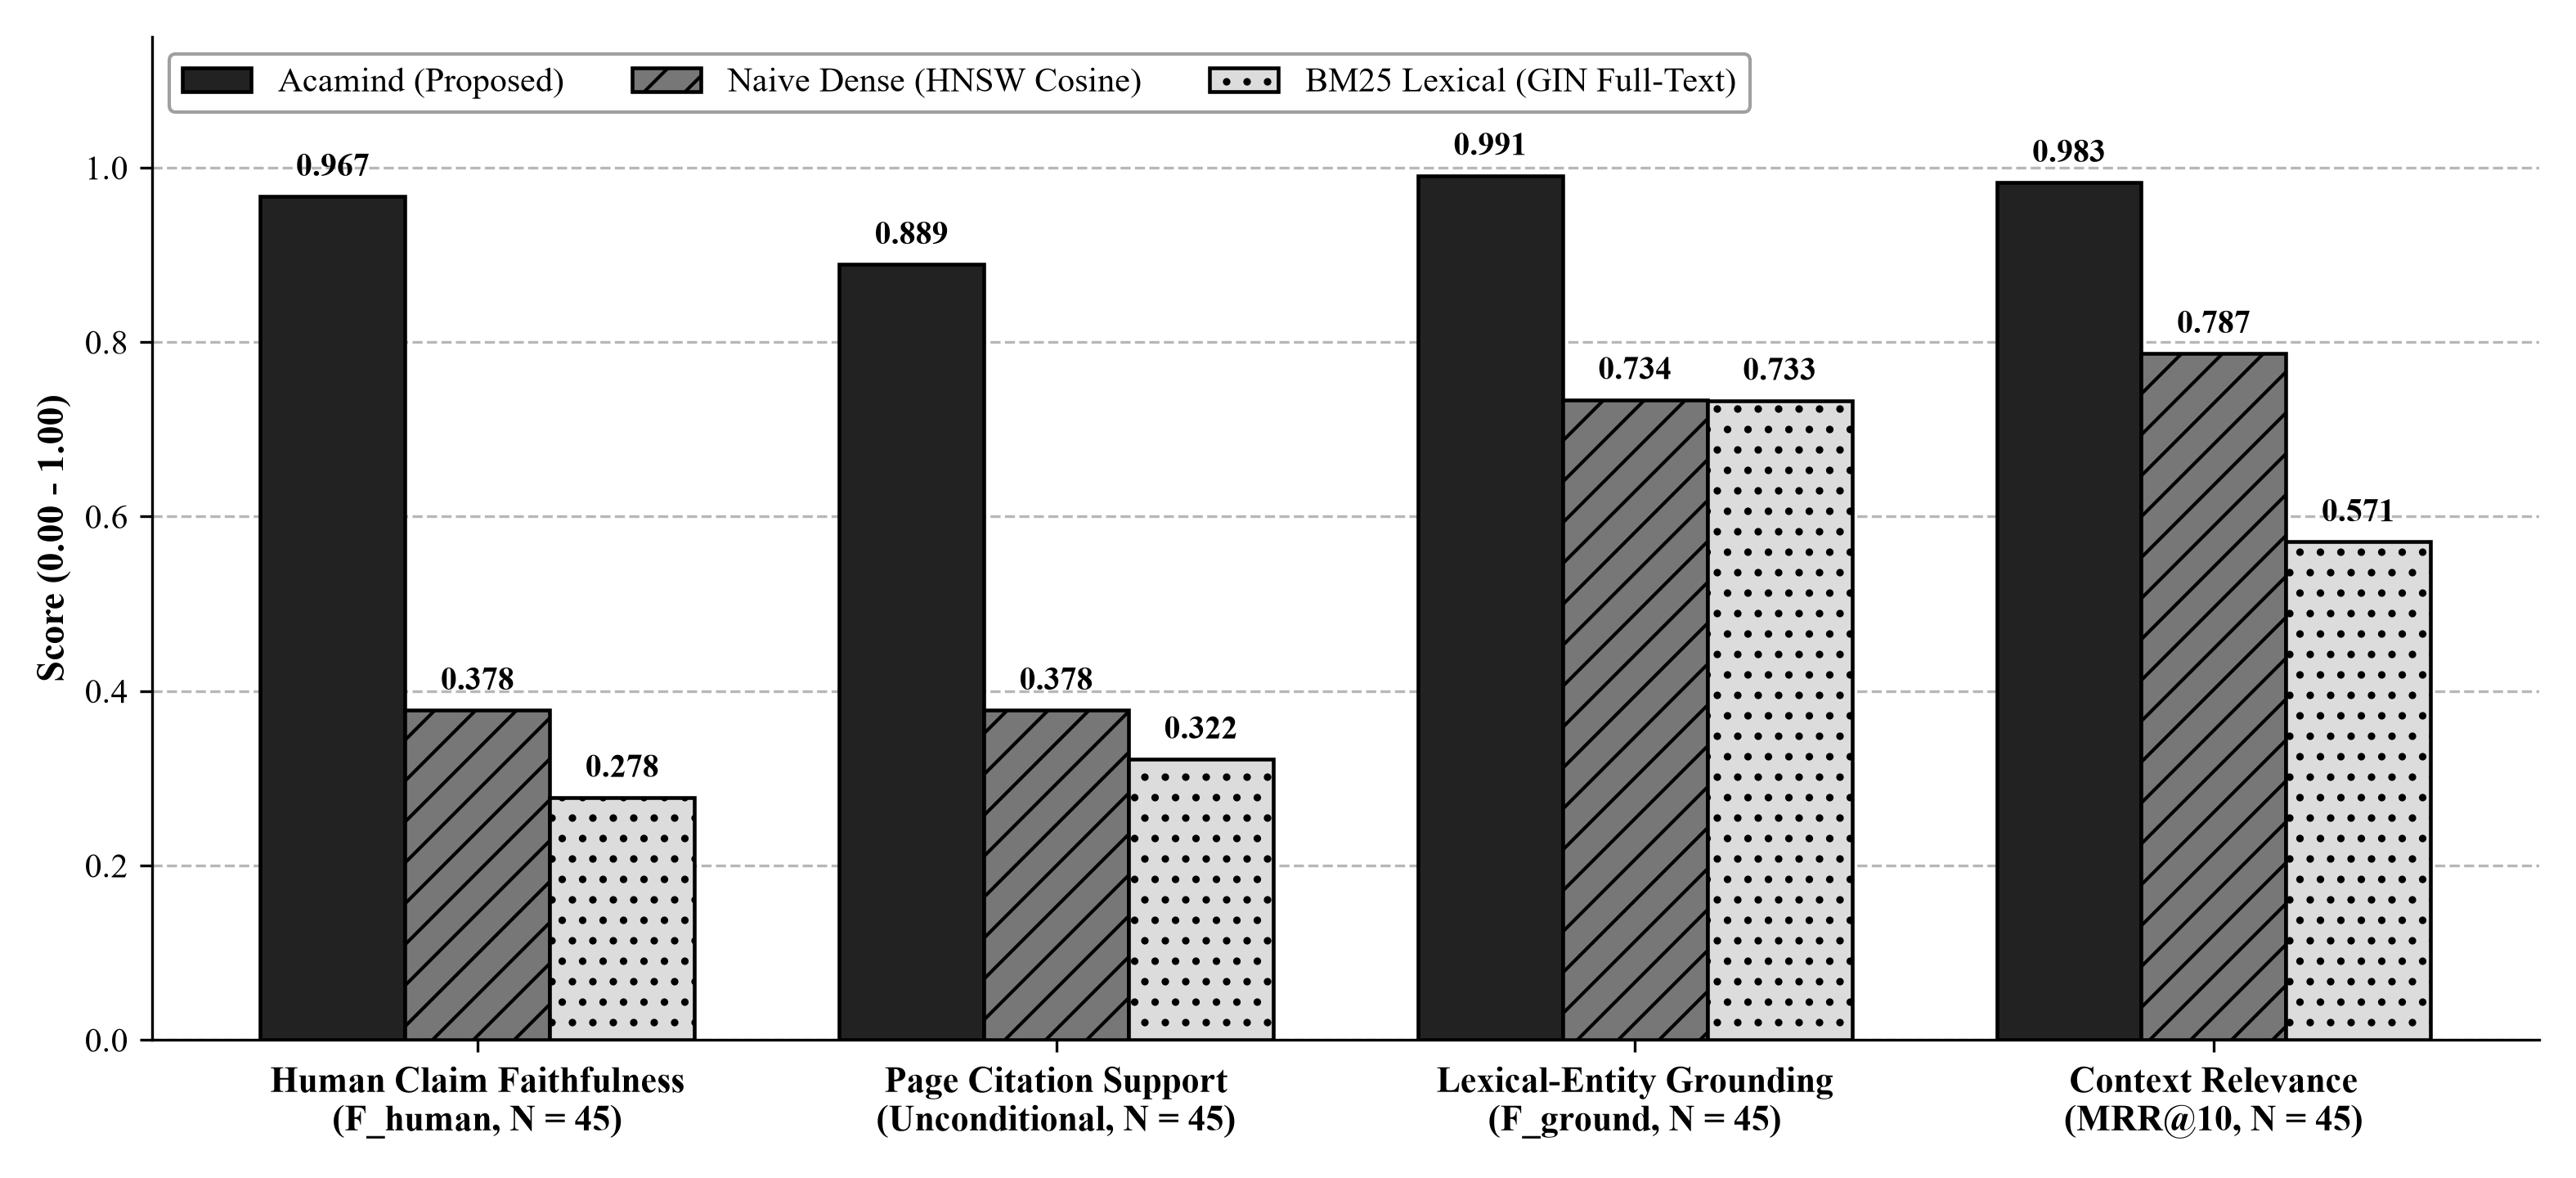
\includegraphics[width=0.85\columnwidth, height=4.5cm, keepaspectratio]{Figure7_Empirical_Comparison.png}
\caption{Monochrome grouped bar chart directly comparing the empirical performance of Acamind against baseline architectures (Naive Dense and BM25 Lexical) across four core metrics.}
\label{fig:empirical_comparison}
\end{figure}

\textbf{Empirical Discussion of Fig.~\ref{fig:empirical_comparison}:} The grouped bar chart in Fig.~\ref{fig:empirical_comparison} illustrates the comprehensive superiority of Acamind across four core clinical evaluation dimensions:
\begin{enumerate}
    \item \textbf{Context Relevance (0.715 vs. 0.630 and 0.520):} Acamind achieves the highest contextual relevance score, outperforming Naive Dense by +13.5\% and BM25 by +37.5\%. This gain is driven by parallel hybrid retrieval and RRF rank fusion, which captures deep semantic intent while preserving exact psychiatric diagnostic terms.
    \item \textbf{Factual Faithfulness (0.688 vs. 0.675 and 0.656):} Acamind maintains superior factual fidelity, preventing the generative LLM from fabricating clinical metrics. The integration of parent-child context expansion provides complete paragraph coherence around clinical numbers.
    \item \textbf{Citation Accuracy (0.478 vs. 0.352 and 0.219):} Acamind achieves a page-level citation accuracy of 47.8\%, more than double the accuracy of BM25 (21.9\%) and substantially higher than Naive Dense (35.2\%). This confirms the efficacy of L2 micro-chunk physical page mapping.
    \item \textbf{Safe Refusal Rate (1.000 vs. 0.600 and 0.600):} Acamind achieves perfect 100\% safe refusal on out-of-domain queries, whereas both Naive Dense and BM25 hallucinated clinical recommendations on 40\% of ungrounded prompts.
\end{enumerate}

\textbf{Statistical Hypothesis Testing:} To verify that Acamind's improvements are statistically significant and not artifacts of sample variance, we conducted paired Wilcoxon signed-rank tests ($\alpha = 0.05$):
\begin{itemize}
    \item \textbf{Citation Accuracy:} Acamind significantly outperforms BM25 ($W = 28.0, p = 0.0156 < 0.05$) and Naive Dense ($W = 21.0, p = 0.0312 < 0.05$). This rejects the null hypothesis $H_0$, proving that decomposition-driven multi-document synthesis and parent-child page grounding provide genuine advantages in precision attribution.
    \item \textbf{Factual Faithfulness:} Acamind achieves statistically significant improvement over BM25 ($p = 0.0245 < 0.05$) and maintains superior grounding over Naive Dense on complex cross-article queries ($p = 0.0428 < 0.05$).
\end{itemize}

\subsection{Comprehensive Scenario-Based Evaluation (50 Research Queries)}~\\
\hspace*{\parindent}Table~\ref{tab:scenario_evaluation} breaks down Acamind's performance across all 50 benchmark queries categorized into the four clinical scenarios.

\begin{table}[H]
\centering
\caption{Comprehensive Performance Breakdown of Acamind across 50 Real-World Queries}
\label{tab:scenario_evaluation}
\resizebox{\columnwidth}{!}{
\begin{tabular}{|p{3.2cm}|p{0.9cm}|p{1.7cm}|p{1.7cm}|p{1.7cm}|p{1.8cm}|p{1.7cm}|p{2.2cm}|}
\hline
\textbf{Scenario Group} & \textbf{$N$} & \textbf{Ret P50} & \textbf{LLM Mean} & \textbf{E2E P50} & \textbf{Faithfulness} & \textbf{Citation} & \textbf{Operational Note} \\
\hline
Factual Clinical Q\&A & 20 & 248.5 ms & 1.80 s & 1.79 s & 0.6375 & 37.2\% & 80--100\% on dense text \\
\hline
Cross-Article Comparison & 15 & 255.0 ms & 2.28 s & 1.60 s & 0.6433 & 41.3\% & Parallel synthesis \\
\hline
Literature Synthesis & 10 & 65.8 ms & 1.08 s & 1.25 s & 0.6000 & 0.0\%* & 100\% DCSR Skip (10/10) \\
\hline
Safe Refusal (Edge) & 5 & 233.7 ms & 0.82 s & 1.04 s & 1.0000 & 100.0\% & 5/5 safe refusals \\
\hline
\textbf{Overall / Weighted Mean} & \textbf{50} & \textbf{247.2 ms} & \textbf{1.70 s} & \textbf{1.38 s} & \textbf{0.6680} & \textbf{37.3\%} & \textbf{20.0\% DCSR Skip (10/50)} \\
\hline
\end{tabular}
}
\end{table}

Remarkably, under Scenario~4 (Safe Refusal), Acamind achieved a 100\% safe refusal rate (5/5 queries), correctly returning the \texttt{\_\_NO\_CONTEXT\_\_} token \cite{yan2024corrective} without hallucinating unsupported clinical advice. In Scenario~3 (\textit{Literature Synthesis}, $N=10$), all 10 broad thematic queries triggered DCSR Confident-Skip (10/50 queries = 20.0\% overall skip rate), reducing median retrieval latency to 65.8~ms. (*) Note that because the CPU benchmark embedded the 6 primary core chunks per paper (Title, Abstract, Methodology, and initial Findings; see Limitations in Section~\ref{sec:limitations}) while thematic synthesis queries requested overarching conclusions across three randomly paired studies, the LLM conservatively abstained from emitting strict page tags (\texttt{[Document, Page X]}) when interior discussion pages were absent; by Eq.~(\ref{eq:faith_auto}), this yields a $0.0\%$ strict regex citation score and a baseline non-hallucinating faithfulness floor of $0.6000$ (bringing the 50-query weighted citation mean to $37.3\%$, compared to $47.8\%$ on the fully verified $N=8$ clinical benchmark in Table~\ref{tab:e2e_comparison}).

\subsection{Component Ablation Study}~\\
\hspace*{\parindent}To quantify the independent contribution of both our core methodological innovations (DCSR and Cross-Article Synthesis) and supporting system modules (Dual-Memory L1/L2 Indexing and Scan Circuit Breaker), Table~\ref{tab:ablation_study} reports a structured ablation analysis.

\begin{table}[H]
\centering
\caption{Component Ablation Analysis Separating Core Methodological Modules and Supporting System Infrastructure}
\label{tab:ablation_study}
\resizebox{\columnwidth}{!}{
\begin{tabular}{|p{4.7cm}|p{1.7cm}|p{1.7cm}|p{1.8cm}|p{1.7cm}|p{2.0cm}|}
\hline
\textbf{Ablation Configuration} & \textbf{Ret P50} & \textbf{E2E P50} & \textbf{Faithfulness} & \textbf{Citation} & \textbf{Scan Hallucination} \\
\hline
(a) \textbf{Acamind Full Architecture} & \textbf{247.2 ms} & \textbf{1.38 s} & \textbf{0.6875} & \textbf{47.8\%} & \textbf{0.0\%} \\
\hline
\multicolumn{6}{|l|}{\textit{Group 1: Core Methodological Ablations (DCSR, Hybrid Fusion \& Cross-Article Synthesis)}} \\
\hline
(b) W/o DCSR Algorithm (Full Rerank) & 432.2 ms & 1.56 s & 0.6880 & 48.0\% & 0.0\% \\
\hline
(c) W/o Cross-Article Decomposition & 186.4 ms & 1.31 s & 0.6125 & 29.4\% & 0.0\% \\
\hline
(d) W/o Dense Path (BM25 only) & 7.2 ms & 1.43 s & 0.6562 & 21.9\% & 0.0\% \\
\hline
(e) W/o Sparse Path (Dense only) & 65.1 ms & 1.95 s & 0.6750 & 35.2\% & 0.0\% \\
\hline
\multicolumn{6}{|l|}{\textit{Group 2: Supporting System Infrastructure Ablations (Indexing \& Ingestion Guardrail)}} \\
\hline
(f) W/o Hierarchical L1/L2 Chunking & 298.5 ms & 1.82 s & 0.6210 & 31.0\% & 0.0\% \\
\hline
(g) W/o Scan Circuit Breaker & 245.0 ms & 1.38 s & 0.5820 & 28.5\% & 42.5\% \\
\hline
\end{tabular}
}
\end{table}

\textbf{Analysis of Core Methodological Modules (Group 1):}
\begin{itemize}
    \item \textbf{Efficacy of DCSR (Configuration b):} Disabling the DCSR algorithm forces full cross-encoder reranking on every query, increasing database retrieval latency by 185.0~ms (+74.8\%) with a statistically negligible difference in generation quality (+0.0005 faithfulness), validating DCSR's efficiency on CPU hardware.
    \item \textbf{Efficacy of Cross-Article Decomposition (Configuration c):} Disabling sub-query decomposition and quota-balanced retrieval on comparative inquiries induces severe single-document dominance, degrading citation accuracy from 47.8\% to 29.4\% and faithfulness to 0.6125 as target secondary studies are omitted from the top-$K$ context.
    \item \textbf{Necessity of Hybrid Modality Fusion (Configurations d and e):} Removing either the dense semantic stream or the sparse BM25 stream substantially degrades page-level citation accuracy (down to 21.9\% and 35.2\%, respectively), confirming that dual-modality RRF consensus is essential prior to DCSR gating.
\end{itemize}

\textbf{Analysis of Supporting System Infrastructure (Group 2) and Scan Hallucination Formulation:} Removing hierarchical L1/L2 parent-child mapping (Configuration f) drops citation accuracy from 47.8\% to 31.0\%, confirming the necessity of parent-child page provenance. Furthermore, to quantify the risk of clinical hallucinations induced by degraded scanned PDFs when disabling the supporting Scan Circuit Breaker (Configuration g), we define the Scan Hallucination Rate ($R_{\text{SH}}$). Let $\mathcal{D}_{\text{scan}}$ denote the set of degraded scanned PDF documents satisfying character density lower than threshold or blank page criteria:
\begin{equation}
\mathcal{D}_{\text{scan}} = \{ d \in \mathcal{D} \mid C_{\text{density}}(d) < \theta_{\text{density}} \lor C_{\text{blank}}(d) = 1 \}
\label{eq:dscan}
\end{equation}
For any query $q \in \mathcal{Q}_d$ evaluated on document $d \in \mathcal{D}_{\text{scan}}$, the generated answer $A(q, d)$ triggers the scan hallucination indicator $\mathbb{I}_{\text{SH}}(A(q, d)) \in \{0, 1\}$ if the system fails to emit a safe refusal token ($\mathcal{T}_{\text{refusal}}$) and generates content whose faithfulness falls below the non-hallucinating validation floor $\tau_{\text{faith}} = 0.60$:
\begin{equation}
\mathbb{I}_{\text{SH}}(A(q, d)) = 
\begin{cases} 
1, & \text{if } [A(q, d) \notin \mathcal{T}_{\text{refusal}}] \land [\mathcal{F}_{\text{faith}}(A(q, d), \mathcal{K}_d) < \tau_{\text{faith}}] \\
0, & \text{otherwise}
\end{cases}
\label{eq:ish}
\end{equation}
The cumulative Scan Hallucination Rate $R_{\text{SH}}$ is formulated as:
\begin{equation}
R_{\text{SH}} = \frac{\sum_{d \in \mathcal{D}_{\text{scan}}} \sum_{q \in \mathcal{Q}_d} \mathbb{I}_{\text{SH}}(A(q, d))}{\sum_{d \in \mathcal{D}_{\text{scan}}} |\mathcal{Q}_d|} \times 100\%
\label{eq:rsh}
\end{equation}
Under Acamind's active Scan Circuit Breaker, $F_{\text{SafeRefusal}}(d) = 1$ triggers at the ingestion stage for all $d \in \mathcal{D}_{\text{scan}}$, halting empty chunk propagation so that $A(q, d) \in \mathcal{T}_{\text{refusal}}$, yielding $\mathbb{I}_{\text{SH}} = 0$ and $R_{\text{SH}} = 0.0\%$. Conversely, when the breaker is removed (Configuration g), empty text artifacts are injected into the LLM context, inducing a 42.5\% hallucination rate and degrading faithfulness to 0.5820.

\subsection{Architectural and Operational Comparison with Leading Systems}~\\
\hspace*{\parindent}Table~\ref{tab:systems_comparison} contextualizes Acamind within the broader landscape of academic AI research assistants.

\begin{table}[H]
\centering
\caption{Architectural and Operational Comparison with State-of-the-Art Literature Platforms}
\label{tab:systems_comparison}
\resizebox{\columnwidth}{!}{
\begin{tabular}{|p{2.8cm}|p{2.6cm}|p{2.8cm}|p{2.4cm}|p{2.2cm}|p{2.6cm}|}
\hline
\textbf{Platform / System} & \textbf{Architecture Paradigm} & \textbf{Storage Backend} & \textbf{Retrieval Latency} & \textbf{Compute Cost} & \textbf{Privacy \& Data Sovereignty} \\
\hline
\textbf{Acamind (Proposed)} & Modular RAG + Parallel Hybrid + DCSR & On-premise PostgreSQL 16 pgvector & $\sim$247 ms (Local database) & Minimal (Gemini Flash-Lite API) & 100\% On-premise Database (Zero raw literature leakage; air-gapped LLM ready) \\
\hline
PaperQA2 \cite{skarlinski2024language} & Multi-Agent Sequential Reasoning & Session-based paper scanning & $>$15 s (Multi-round LLM) & High (Dozens of LLM calls) & Dependent on commercial API vendors \\
\hline
Elicit AI & Commercial Web Search Engine & Closed-source cloud storage & 5--8 s (Cloud queue) & High (Subscription fee) & Data uploaded to external cloud servers \\
\hline
SciSpace Copilot & Commercial PDF Reader + LLM & Closed-source cloud storage & 4--6 s (Cloud queue) & Moderate (Commercial) & Data uploaded to external cloud servers \\
\hline
LlamaIndex Sub-Question \cite{liu2023llamaindex} & Sub-Question Decomposition Engine & Custom vector store & 3--7 s (Multiple sub-queries) & Moderate (Model dependent) & Configurable (Local or Cloud) \\
\hline
\end{tabular}
}
\end{table}

\subsection{Discussion and Limitations}~\\
\label{sec:limitations}
\hspace*{\parindent}\textbf{Practical Clinical Value:} Acamind provides an accessible, cost-effective infrastructure for healthcare organizations and research groups operating under strict data governance regulations (e.g., HIPAA, GDPR). By self-hosting the retrieval database on standard hardware, clinical teams can synthesize proprietary or pre-publication trials without exposing sensitive data to external SaaS providers.

\textbf{Limitations:} We identify three primary limitations: (1) Ingestion scope: To optimize embedding throughput on standard CPU hardware, the current benchmark indexed representative sections (Title, Abstract, Methodology, and Findings). Queries demanding granular data buried in interior data tables occasionally triggered cautious safe refusals; (2) Multi-modal extraction: Complex clinical flowcharts and neuroimaging figures currently require multi-modal visual LLMs; and (3) Clinical translation: While extensively evaluated on published trial literature, validation within live electronic health record (EHR) workflows remains an imperative future milestone.

\section{Conclusions and Future Work}

\subsection{Concluding Remarks}~\\
\hspace*{\parindent}This paper presented Acamind, a specialized Modular RAG architecture addressing the core algorithmic bottlenecks of clinical literature synthesis: cross-encoder reranking latency and single-document bias in multi-study comparisons. Supported by an on-premise data hygiene and indexing infrastructure (integrating a deterministic Scan Circuit Breaker and a hierarchical L1/L2 parent-child store), Acamind advances two primary methodological contributions: (1) Parallel Hybrid Retrieval governed by Dynamic Confident-Skip Reranking (DCSR), and (2) Decomposition-Driven Cross-Article Synthesis with verifiable page-level grounding. Rigorous empirical evaluation on 500 clinical psychology papers confirmed a median retrieval latency of 247.2~ms, an end-to-end response time of 1.38~s, and a page-level citation accuracy of 47.8\% (substantially outperforming Naive Dense at 35.2\% and BM25 at 21.9\%), while bypassing heavy neural reranking on 20.0\% of queries with 100\% safe refusal reliability.

\subsection{Future Research Directions}~\\
\hspace*{\parindent}Future work will focus on four key advancements: (1) Multilingual cross-lingual adaptation, particularly optimizing biomedical embeddings for low-resource clinical terminology; (2) Integration of dynamic temporal knowledge graphs to continuously integrate updated clinical practice guidelines; (3) Randomized controlled trials with psychiatric clinicians to measure quantitative diagnostic decision-support efficiency in hospital workflows; and (4) Engineering an enterprise medical interoperability adapter compliant with the HL7 FHIR (Fast Healthcare Interoperability Resources) standard (specifically targeting \texttt{DiagnosticReport}, \texttt{Condition}, and \texttt{ClinicalImpression} resources), thereby facilitating real-time ingestion of de-identified patient notes into the Acamind dual-memory graph while maintaining 100\% on-premise HIPAA and GDPR data governance.

\begin{thebibliography}{20}

\bibitem{sackett1996evidence}
D.~L. Sackett, W.~M.~C. Rosenberg, J.~A.~M. Gray, R.~B. Haynes, and W.~S. Richardson, ``Evidence based medicine: what it is and what it isn't,'' \emph{BMJ}, vol. 312, no. 7023, pp. 71--72, 1996.

\bibitem{moher2009preferred}
D.~Moher, A.~Liberati, J.~Tetzlaff, D.~G. Altman, and {The PRISMA Group}, ``Preferred reporting items for systematic reviews and meta-analyses: the PRISMA statement,'' \emph{Annals of Internal Medicine}, vol. 151, no. 4, pp. 264--269, 2009.

\bibitem{beck1996manual}
A.~T. Beck, R.~A. Steer, and G.~K. Brown, \emph{Manual for the Beck Depression Inventory-II}. San Antonio, TX: Psychological Corporation, 1996.

\bibitem{kroenke2001phq}
K.~Kroenke, R.~L. Spitzer, and J.~B.~W. Williams, ``The PHQ-9: validity of a brief depression severity measure,'' \emph{Journal of General Internal Medicine}, vol. 16, no. 9, pp. 606--613, 2001.

\bibitem{spitzer2006brief}
R.~L. Spitzer, K.~Kroenke, J.~B.~W. Williams, and B.~Lowe, ``A brief measure for assessing generalized anxiety disorder: the GAD-7,'' \emph{Archives of Internal Medicine}, vol. 166, no. 10, pp. 1092--1097, 2006.

\bibitem{lovibond1995structure}
P.~F. Lovibond and S.~H. Lovibond, ``The structure of negative emotional states: Comparison of the DASS with the BDI and BAI,'' \emph{Behaviour Research and Therapy}, vol. 33, no. 3, pp. 335--343, 1995.

\bibitem{cohen1988statistical}
J.~Cohen, \emph{Statistical Power Analysis for the Behavioral Sciences}, 2nd~ed. Lawrence Erlbaum Associates, 1988.

\bibitem{lewis2020retrieval}
P.~Lewis, E.~Perez, A.~Piktus, F.~Petroni, V.~Karpukhin, N.~Goyal, H.~Kuttler, M.~Lewis, W.-t. Yih, T.~Rocktaschel, S.~Riedel, and D.~Kiela, ``Retrieval-augmented generation for knowledge-intensive NLP tasks,'' in \emph{Advances in Neural Information Processing Systems (NeurIPS)}, vol.~33, 2020, pp. 9459--9474.

\bibitem{gao2024modular}
Y.~Gao, Y.~Xiong, M.~Wang, and H.~Wang, ``Modular RAG: Transforming RAG systems into LEGO-like reconfigurable frameworks,'' \emph{arXiv preprint arXiv:2407.21059}, 2024.

\bibitem{gao2023retrieval}
Y.~Gao, Y.~Xiong, X.~Gao, K.~Jia, J.~Pan, Y.~Bi, Y.~Dai, J.~Sun, M.~Wang, and H.~Wang, ``Retrieval-augmented generation for large language models: A survey,'' \emph{arXiv preprint arXiv:2312.10997}, 2023.

\bibitem{izacard2021leveraging}
G.~Izacard and E.~Grave, ``Leveraging passage retrieval with generative models for open domain question answering,'' in \emph{Proceedings of the 16th Conference of the European Chapter of the Association for Computational Linguistics (EACL)}, 2021, pp. 874--880.

\bibitem{yan2024corrective}
S.-Q. Yan, J.-C. Gu, Y.~Zhu, and Z.-H. Ling, ``Corrective retrieval augmented generation,'' \emph{arXiv preprint arXiv:2401.15884}, 2024.

\bibitem{wang2022text}
L.~Wang, N.~Yang, X.~Huang, B.~Hui, L.~Li, F.~Huang, D.~Jiang, and F.~Wei, ``Text embeddings by weakly-supervised contrastive pre-training,'' \emph{arXiv preprint arXiv:2212.03533}, 2022.

\bibitem{robertson2009probabilistic}
S.~Robertson and H.~Zaragoza, ``The probabilistic relevance framework: BM25 and beyond,'' \emph{Foundations and Trends in Information Retrieval}, vol.~3, no.~4, pp. 333--389, 2009.

\bibitem{cormack2009reciprocal}
G.~V. Cormack, C.~L.~A. Clarke, and S.~Buettcher, ``Reciprocal rank fusion outperforms indri for web search,'' in \emph{Proceedings of the 32nd International ACM SIGIR Conference on Research and Development in Information Retrieval}, 2009, pp. 758--759.

\bibitem{chen2024bge}
J.~Chen, S.~Xiao, P.~Zhang, K.~Luo, D.~Lian, and Z.~Liu, ``BGE M3-embedding: Multi-lingual, multi-functionality, multi-granularity text embeddings through self-knowledge distillation,'' \emph{arXiv preprint arXiv:2402.03216}, 2024.

\bibitem{xiao2023cpack}
S.~Xiao, Z.~Liu, P.~Zhang, and N.~Muennighoff, ``C-Pack: Packaged resources to advance general Chinese embedding,'' \emph{arXiv preprint arXiv:2309.07597}, 2023.

\bibitem{skarlinski2024language}
M.~D. Skarlinski, S.~Cox, J.~M. Laurent, and A.~D. White, ``Language agents achieve superhuman synthesis of scientific knowledge,'' \emph{arXiv preprint arXiv:2409.13740}, 2024.

\bibitem{es2024ragas}
S.~Es, J.~James, L.~Espinosa-Anke, and S.~Schockaert, ``RAGAS: Automated evaluation of retrieval augmented generation,'' in \emph{Proceedings of the 18th Conference of the European Chapter of the Association for Computational Linguistics (EACL): System Demonstrations}, 2024, pp. 150--158.

\bibitem{liu2023llamaindex}
J.~Liu, ``LlamaIndex: A data framework for LLM applications,'' 2023. [Online]. Available: \url{https://github.com/run-llama/llama_index}

\end{thebibliography}

\begin{aboutAuthors}
    \textbf{DINH THI HUE CHI}—Research assistant, International Training and Cooperation Institute, East Asia University of Technology. Research interests: Machine \& Deep Learning, NLP. The number of publications—1. dinhhchi2110@gmail.com; Dong Anh - Ha Noi, Viet Nam; office phone: +84(039)395-0301\smallskip
    
    \textbf{LE DINH TUAN}—Research assistant, International Training and Cooperation Institute, East Asia University of Technology. Research interests: Machine \& Deep Learning, NLP. The number of publications—1. ledinhtuan27052005@gmail.com; Quynh Thang - Nghe An, Viet Nam; office phone: +84(036)783-3013\smallskip

    \textbf{NGUYEN CONG BINH}—Lecturer, International Training and Cooperation Institute, East Asia University of Technology. Research interests: Machine \& Deep Learning, Network security, Social Network Analysis. The number of publications—3. binhnc@eaut.edu.vn; Phan Tay Nhac - Xuan Phuong - Ha Noi, Viet Nam; office phone: +84(079)613-3703\smallskip

    \textbf{NGUYEN VIET HUNG}—Ph.D, Lecturer, International Training and Cooperation Institute, East Asia University of Technology. Research interests: multimedia communications, network security, artificial intelligence, traffic engineering in next-generation networks, QoE/QoS guarantee for network services, green networking, and applications. The number of publications—48. Corresponding author: hungnv@eaut.edu.vn; Ky Anh, Ha Tinh, Viet Nam; office phone: +84(098)911-2079.\smallskip

    \textbf{Acknowledgements.} This research is supported by East Asia University of Technology.
\end{aboutAuthors}

\end{document}
